\documentclass[11pt, letterpaper]{article}
\usepackage{amsmath}
\usepackage{caption}
\usepackage{subcaption}
\usepackage{color}
\usepackage{float}
\usepackage{fullpage}
\usepackage{graphicx}
\usepackage{longtable}
\usepackage{multirow}
\usepackage[nottoc]{tocbibind}
\usepackage{subcaption}
\usepackage{url}
\setlength{\pdfpagewidth}{\paperwidth}
\setlength{\pdfpageheight}{\paperheight}

\renewcommand{\captionfont}{\small}

\newcommand{\degrees}{$^{\circ}$ \,}
% \newcommand{\question}[1]{\textbf{#1}}

\begin{document}
\title{A Local Weather Simulation Model and Extentions to the Transaction Model for BigPetStore}
\author{Ronald J. Nowling}

\maketitle

\newpage

\tableofcontents

\newpage

\section{Introduction}
BigPetStore is a family of realistic example applications for the Hadoop and Spark ecosystems based on around synthetic transaction data for a fictional chain of pet stores.  At the heart of BigPetStore is a data generator that implements a model for simulating customer behavior.  The patterns embedded in the data as a result of the model are used as the basis for analytics examples.  The incorporation of additional effects can increase the realism of the data and provide opportunities for adding more examples analyses to BigPetStore.

The data generator model aims to, where possible, incorporate effects based on \emph{ab initio} assumptions of customer behavior.  This has the advantage of making it easy to recover the resulting patterns given knowledge of the assumptions.  As part of our continual effort to expand and improve the model, we want to model the effect of weather patterns on customer purchasing habits.  For example, customers tend to bulk up on items before impending bad weather such as snow storms.  Economic activity also tends to be reduced during cold weather.  A side effect of incorporating the influence of weather in the model is the addition of regional variations in customer purchasing behavior.

Of course, to incorporate the effects of weather into the model, we first need weather data. To support simulation of arbitrary time periods, we decided to develop a simple dynamical model for generating weather data, parameterized by real, historical weather data.

\newpage
\section{Local Weather Model}

\subsection{Data Sources and File Formats}
\textcolor{red}{NOAA C}

\subsection{Temperature}
\subsubsection{Analysis of Real Data} \label{sec:analysis}
To build a model, we need to a set of assumptions governing the behavior of the model.  By analyzing the existing data, we can infer patterns to inform our assumptions.  For the analysis, we'll use the average daily temperatures from South Bend, IN between October, 2011 to October, 2014.

The average daily temperatures are plotted in Figure~\ref{fig:analysis-raw}. We can make a few immediate observations.  First, the temperatures are between -6$^{\circ}$ F and 90$^{\circ}$ F with an average temperature of 50.7$^{\circ}$ F.  Secondly, the temperatures seem to be governed by multiple frequencies, in particular high-frequency components related to daily variations in temperature and low-frequency components related to seasonal variations.  The low-frequency component seems to be periodic and determinstic, while the high-frequency component seems to be stochastic.

The frequency spectra of the temperatures was computed using a Fourier Transform and is plotted in Figure~\ref{fig:analyis-ft}.  The frequency spectra is characterized by a low-frequency signal with a period of 363.3 days and a high amplitude of 23.9 $^{\circ}$ F, a few other low-frequency signals with periods of 1090.0, 545.0, and 272.5 days with higher-than-average amplitudes (2.1 - 3.4 $^{\circ}$ F), and the remaining signals with amplitudes that are somewhat uniformally-distributed (see Table~\ref{tab:analysis-ft-values}).  The high-amplitude, low-frequency signals correspond to the seasonal change we observed in the raw data.  The uniform-amplitude signals are indicative of ``white'' noise which spans all frequencies. 

The autocorrelation of the daily temperatures is given in Figure~\ref{fig:analyis-autocorr}.  The autocorrelation indicates a periodic correlation with a period of approximately a year, which agrees with our observation of a high-amplitude signal with a period of 363.3 days.  The low levels of correlation for small lag times ($<$ days), is indicative of ``white noise,'' which is not be correlated in time. The tendency for the correlation to increase as the time lag increases is likely to be due to the dominance of the low-frequency deterministic component over the all-frequency stochastic noise.

This suggests we may be able to model the temperatures using a low-frequency determistic component plus a ``white''-noise stochastic process.

\begin{table}[H]
  \centering
  \begin{tabular}{c c c c} \hline
  \emph{Frequency (cylces/day)} & \emph{Period(days)} & \emph{Coefficients ($^{\circ}$ F)} & \emph{Amplitudes ($^{\circ}$ F)}\\ \hline
  0.0009 & 1090.0 & $0.4375-3.3216i$ & 3.3503 \\ \hline
  0.0018 & 545.0 & $-0.2102-2.0662i$ & 2.0770 \\ \hline
  0.0028 & 363.3 & $7.8294+22.6238i$ & 23.9402 \\ \hline
  0.0037 & 272.5 & $-2.7955+1.1398i$ & 3.0190 \\ \hline
  0.0046 & 218.0 & $-0.9682-1.2431i$ & 1.5757 \\ \hline
  \end{tabular}
  \caption{}
  \label{tab:analysis-ft-values}
\end{table}

\textcolor{red}{TODO: velocities}

\begin{enumerate}
\item The temperature process is driven by two components: 3-4 signals in the low-frequency regime with amplitudes $>$ than the median amplitude while the other frequencies have amplitudes near the median (FFT).
\item The low-frequency signals are deterministic and sinosidal (autcorrelation).
\item The signals for the remaining frequencies are characterized by a stochastic process (autocorrelation).
\item The derivative of the temperature is normally (Gaussian) distributed (derivative value histogram).
\item The stochastic process appears to be bounded.
\end{enumerate}



\subsubsection{Description of Model}
Based on the properties observed in Section~\ref{sec:analysis}, we can derive a model combining a Fourier series for the low-frequency components and an Orstein-Uhlenbeck process for the noise.

\begin{align}
&\tilde{T}(t) = \frac{1}{2}a_0 + \sum_{n=1}^k a_n \sin\Big(\frac{-2.0 \pi n}{P}\Big) + b_n \cos\Big(\frac{-2.0 \pi n}{P}\Big) + Z(t) \\
&dZ_t = \theta (\mu - Z_t)dt + \sigma dW_t
\end{align}

\begin{table}[H]
  \centering
  \begin{tabular}{c c} \hline
  \emph{Variable} & \emph{Description}\\ \hline
  $\tilde{T}$ & Simulated temperature \\ \hline
  $t$ & time \\ \hline
  $k$ & Order of Fourier Series \\ \hline
  $a_0$ & average temperature \\ \hline
  $a_n$ & \\ \hline
  $b_n$ &  \\ \hline
  $P$ & period  \\ \hline
  $Z_t$ & Ornstein-Uhlenbeck process \\ \hline
  $\theta$ & \\ \hline
  $\mu$ & long-term mean \\ \hline
  $\sigma^2$ & variance of the Wiener process \\ \hline
  $dW(t)$ & Weiner process \\ \hline 
  \end{tabular}
  \caption{Descriptions of variables in the model}
  \label{tab:analysis-ft-values}
\end{table}


\subsubsection{Implementation of the Model}
In implementing the model, we made several decisions.  We decided to use only one Fourier term ($k=1$) with a period $P$ of 365.0 days.  We determined the values of the coefficients $a_0$, $a_1$, and $b_1$ from a Fourier Transform of the real data.  We set the long-term mean $\mu$ to 0 and determined the variance $\sigma^2$ from the distribution of the derivative of the real temperature data.

We chose to numerically integrate the Orstein-Uhlenbeck process $Z(t)$ using the Euler-Maruyama method:

\begin{align}
&Z_{t+1} = - \theta Z_t \Delta t + \sigma \sqrt{\Delta t} X_{t+1} \\
&Z_0 = 0
\end{align}

where $\Delta t$ is the time step (one day) and $X_t \sim N(0, \sigma^2)$.

\subsubsection{Evaluation of Model}

\begin{figure}[H]
  \centering
  \begin{subfigure}[b]{0.45\textwidth}
    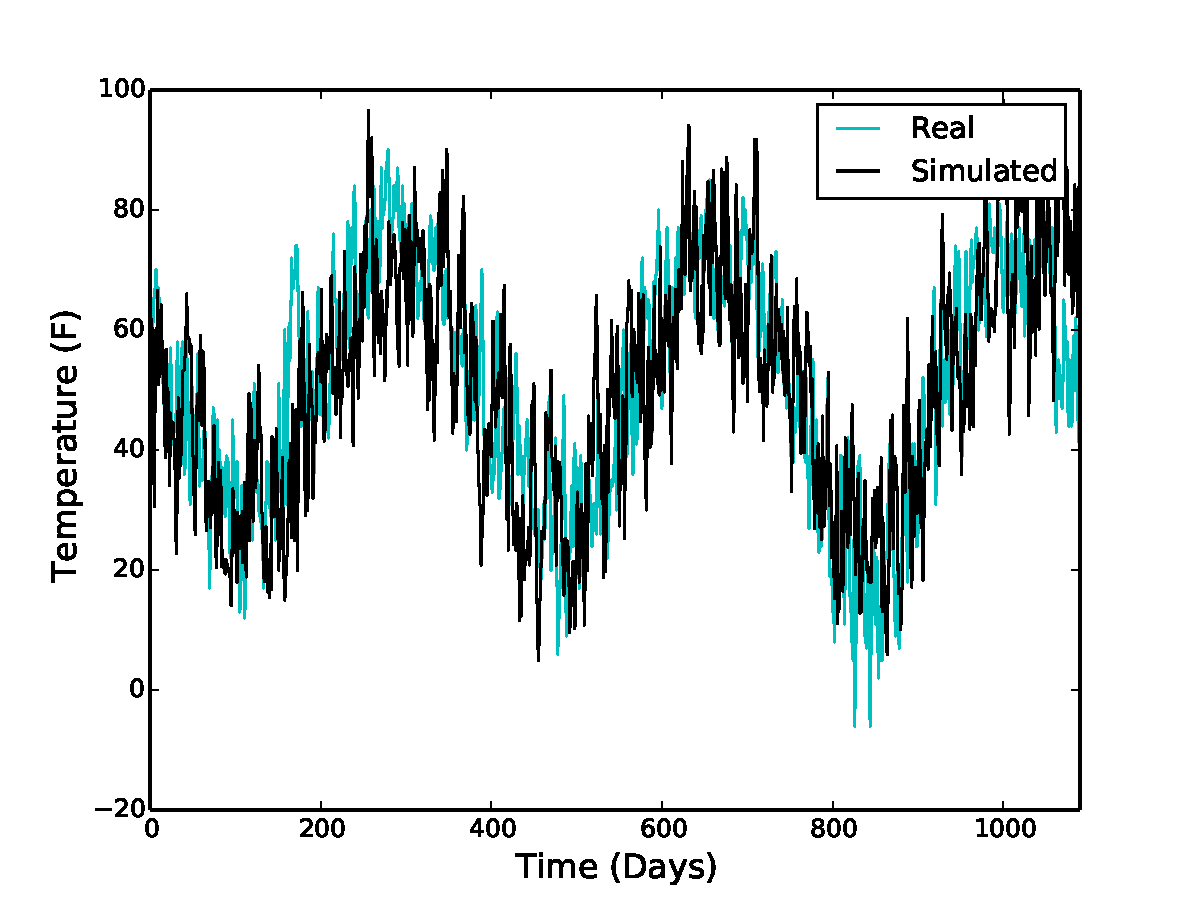
\includegraphics[width=\textwidth]{figures/sim_temp.pdf}
    \label{fig:analysis-raw}
    \caption{Average Daily Temperature}
  \end{subfigure}
  ~
  \begin{subfigure}[b]{0.45\textwidth}
    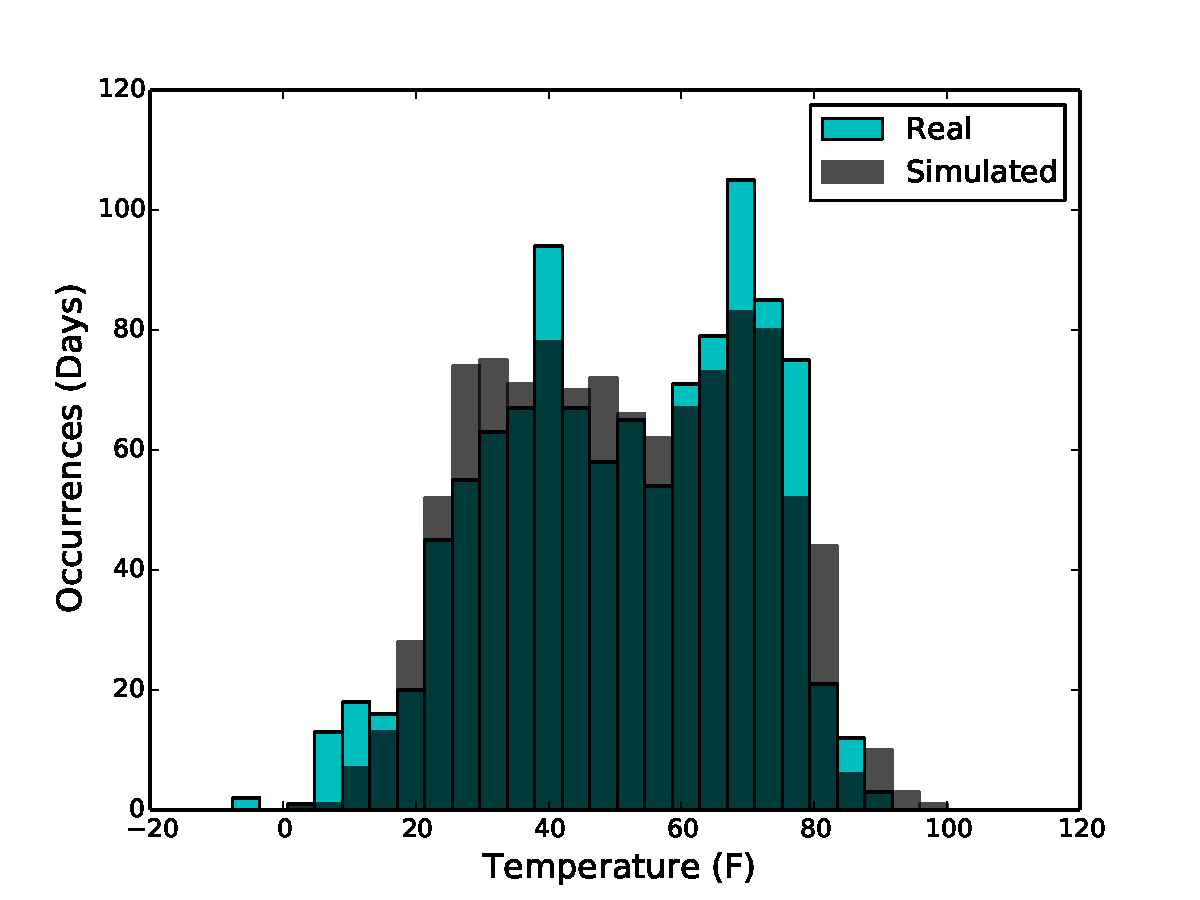
\includegraphics[width=\textwidth]{figures/sim_temp_hist.pdf}
    \caption{Histogram of Temperatures}
  \end{subfigure}
  ~
  \begin{subfigure}[b]{0.45\textwidth}
    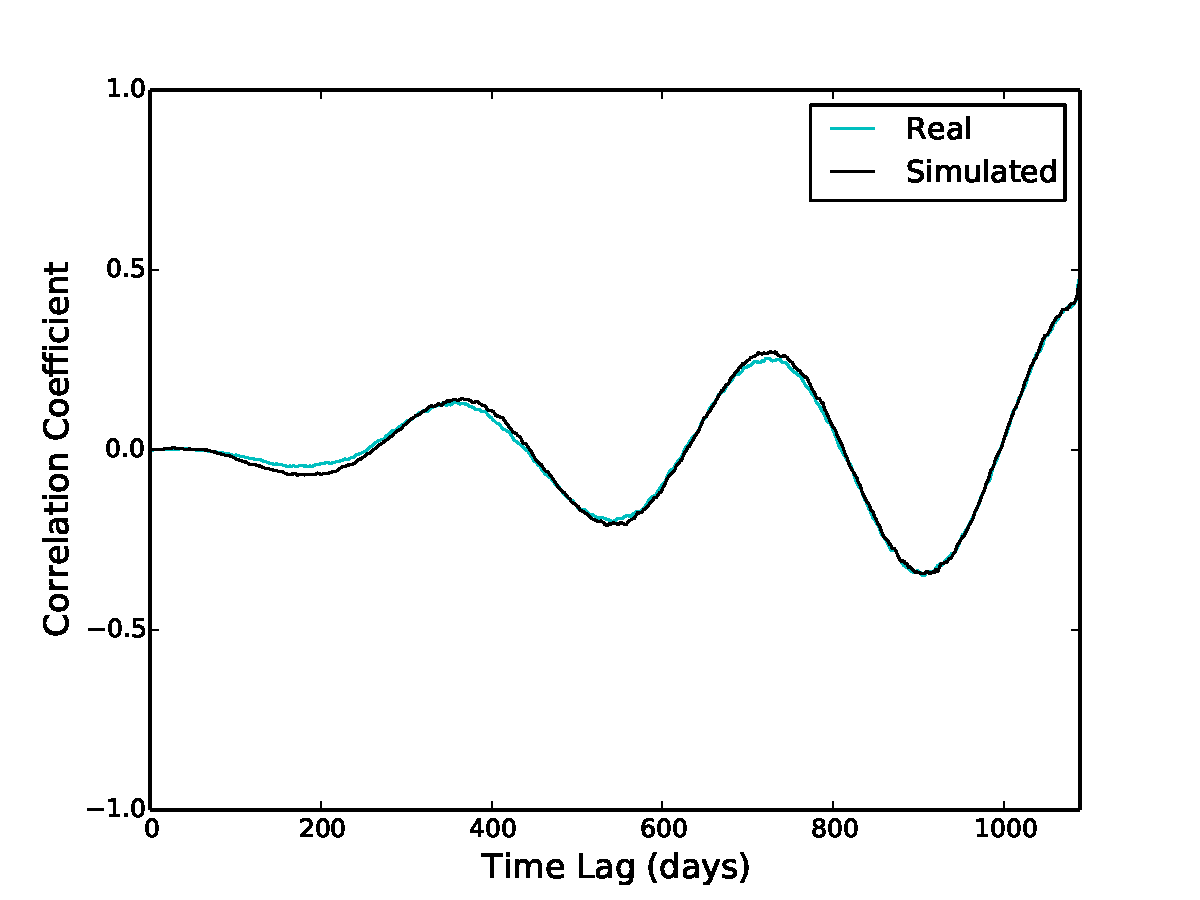
\includegraphics[width=\textwidth]{figures/sim_temp_autocorr.pdf}
    \caption{\label{fig:analysis-autocorr} Autocorrelation}
  \end{subfigure}
  ~
  \begin{subfigure}[b]{0.45\textwidth}
    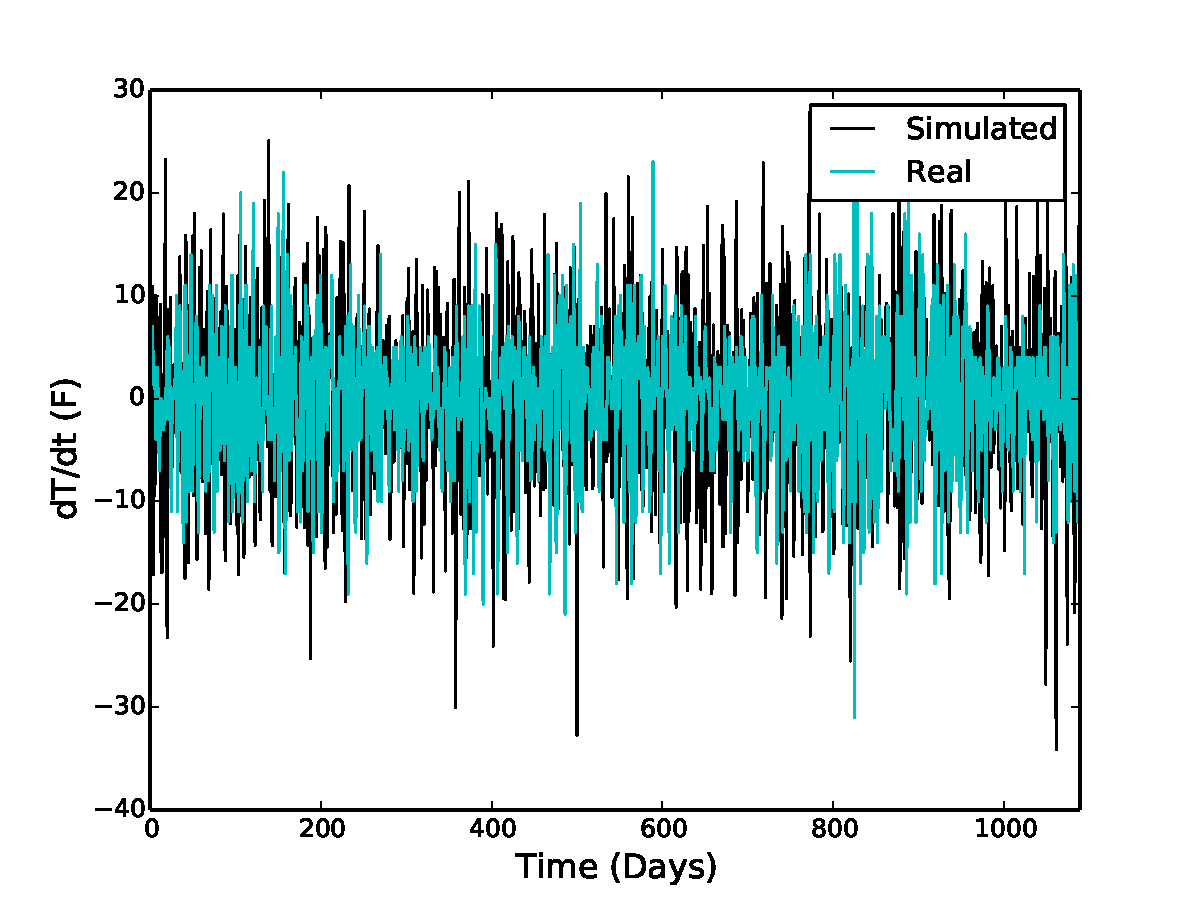
\includegraphics[width=\textwidth]{figures/sim_vel.pdf}
    \caption{\label{fig:analysis-autocorr} Derivative ($dT/dt$) of Temperature}
  \end{subfigure}
  ~
  \begin{subfigure}[b]{0.45\textwidth}
    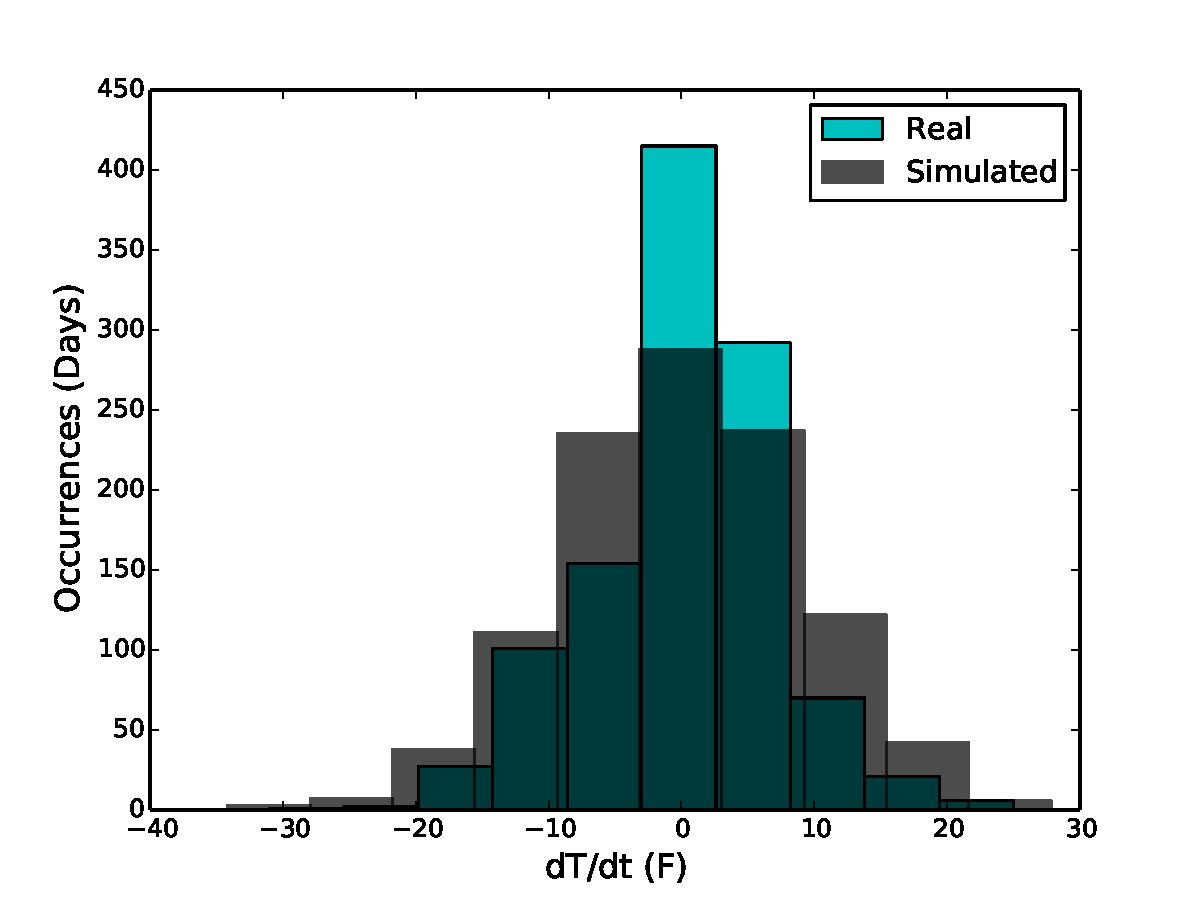
\includegraphics[width=\textwidth]{figures/sim_vel_hist.pdf}
    \caption{\label{fig:analysis-autocorr} Histogram of Derivative ($dT/dt$) of Temperature}
  \end{subfigure}
  %~
  %\begin{subfigure}[b]{0.45\textwidth}
  %  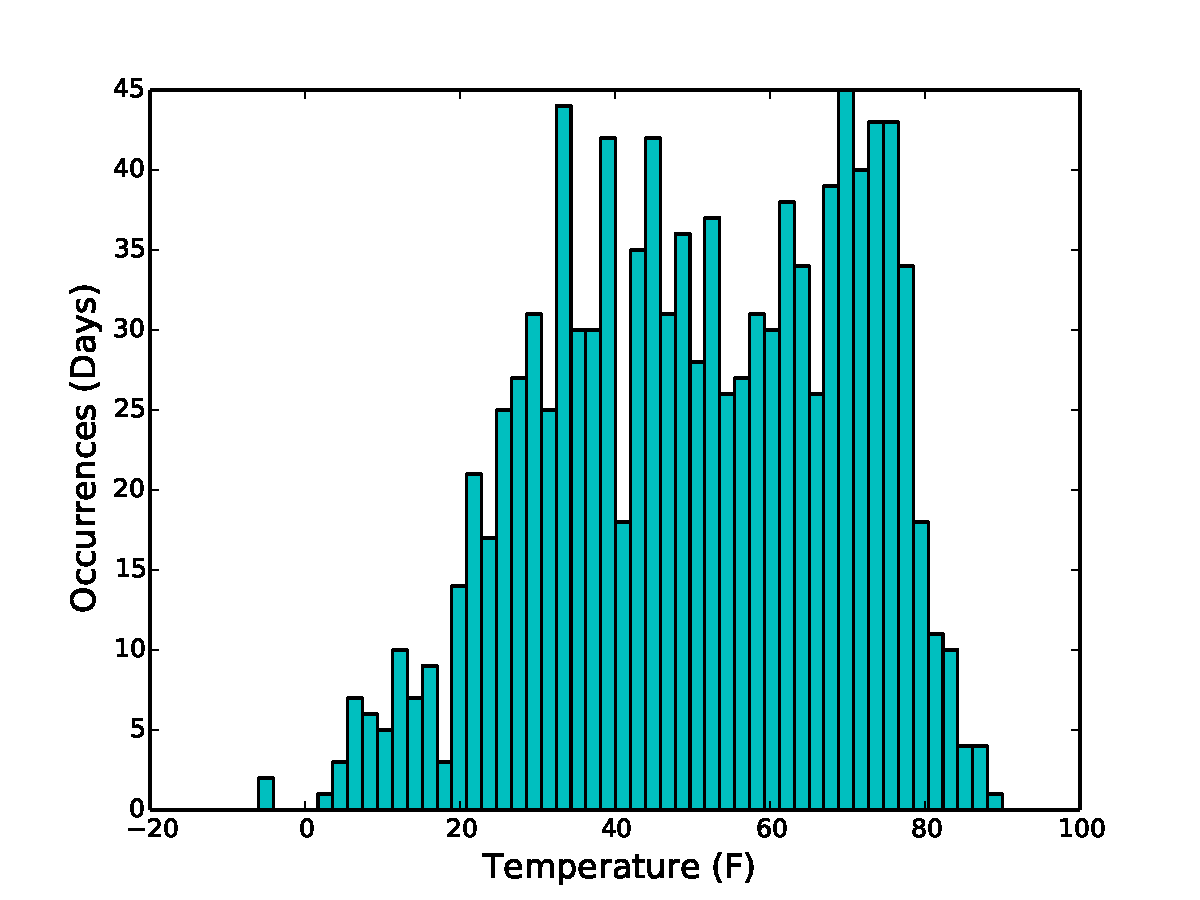
\includegraphics[width=\textwidth]{figures/average_daily_temp_hist.pdf}
  %  \caption{Histogram of Temperatures}
  %\end{subfigure}
  ~
  \begin{subfigure}[b]{0.45\textwidth}
    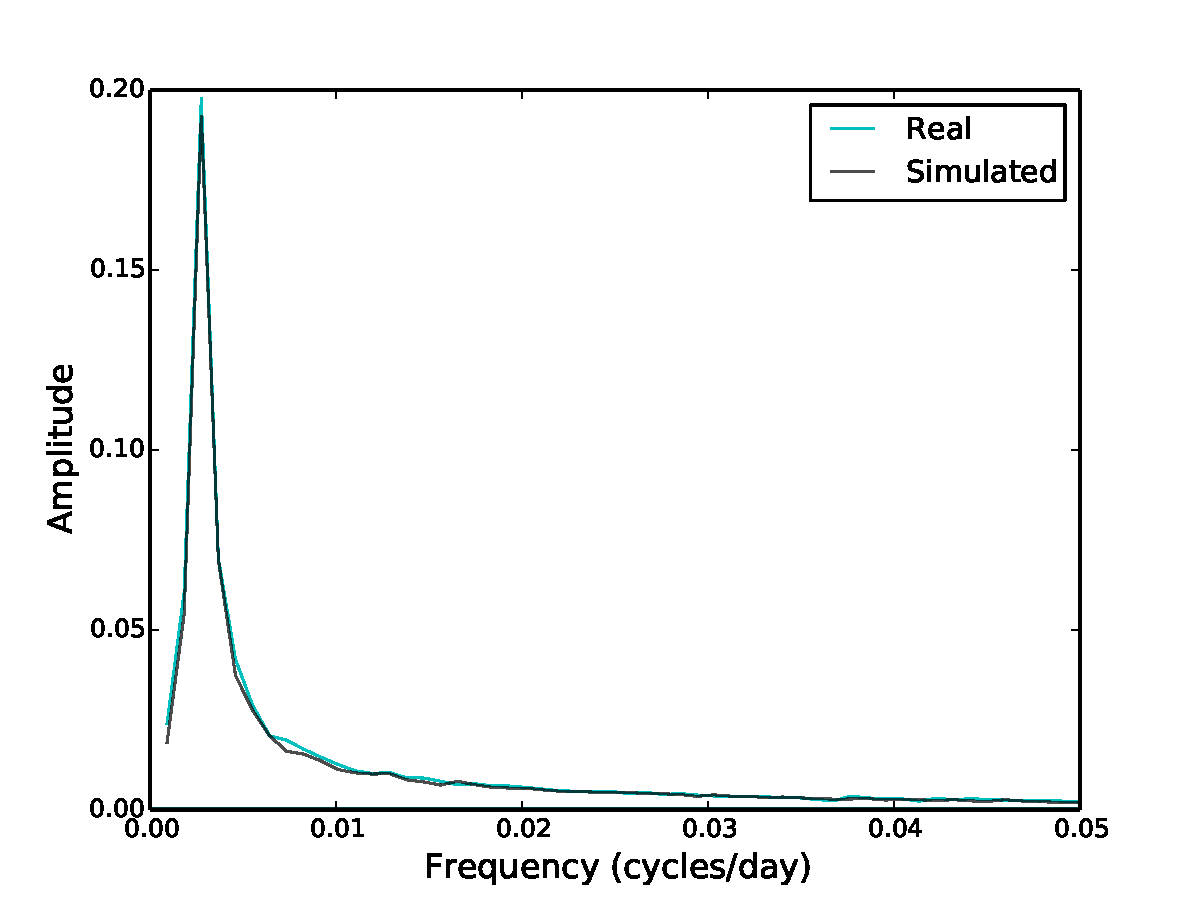
\includegraphics[width=\textwidth]{figures/sim_temp_fft.pdf}
    \label{fig:analysis-ft}
    \caption{Frequency Spectrum}
  \end{subfigure}
  
  \label{fig:analysis}
  \caption{}
\end{figure}

\textcolor{red}{TODO graph of temp histogram}

\subsection{Precipitation}

\subsubsection{Analysis of Real Data}

\begin{enumerate}
\item Precipitation is not correlated in time.  i.e., precipitation is independent day to day
\item Frequencies follow an exponential distribution
\item State (e.g., rain, snow) depends on temperature
\end{enumerate}

\subsubsection{Description of Model}

Precipitation frequency follows an exponential distribution:
\begin{equation}
p(P_t | t) = \lambda \exp(-\lambda P_t)
\end{equation}

Precipitation amounts for a given day are determined by sampling a value for $P_t$ from $p(P_t | t)$.  The precipitation is given as ``water equivalent,'' meaning the amount of liquid water.

Snow-rain ratio is modeled by a logistic function $r(t)$ of the temperature:

\begin{equation}
r(T) = \frac{1}{1 + \exp(-a (T - b))}
\end{equation}

The amount of snowfall must be calculated from the precipitation $r_t$ and percentage of snowfall $r(T)$.  Assuming that snow has a density that is $1/10$ that of water, the amunt of snowfall is given by:

\begin{equation}
s(t) = 10.0 \, (1 - r(T_t)) \, P_t
\end{equation}

\subsubsection{Implementation of the Model}

\subsubsection{Evaluation of Model}

\begin{figure}[H]
  \centering
  \begin{subfigure}[b]{0.45\textwidth}
    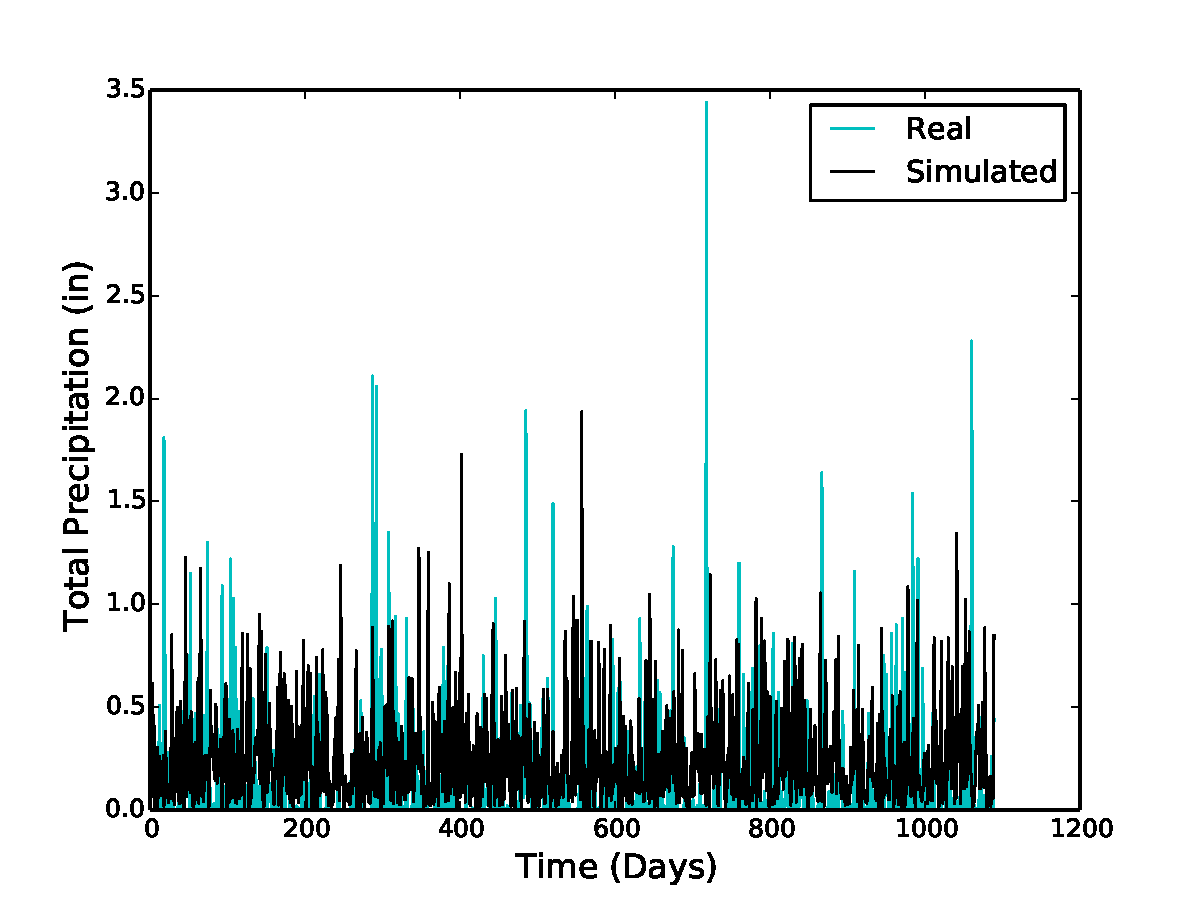
\includegraphics[width=\textwidth]{figures/daily_precip.pdf}
    \label{fig:analysis-raw}
    \caption{Daily Precipitation}
  \end{subfigure}
  ~
  \begin{subfigure}[b]{0.45\textwidth}
    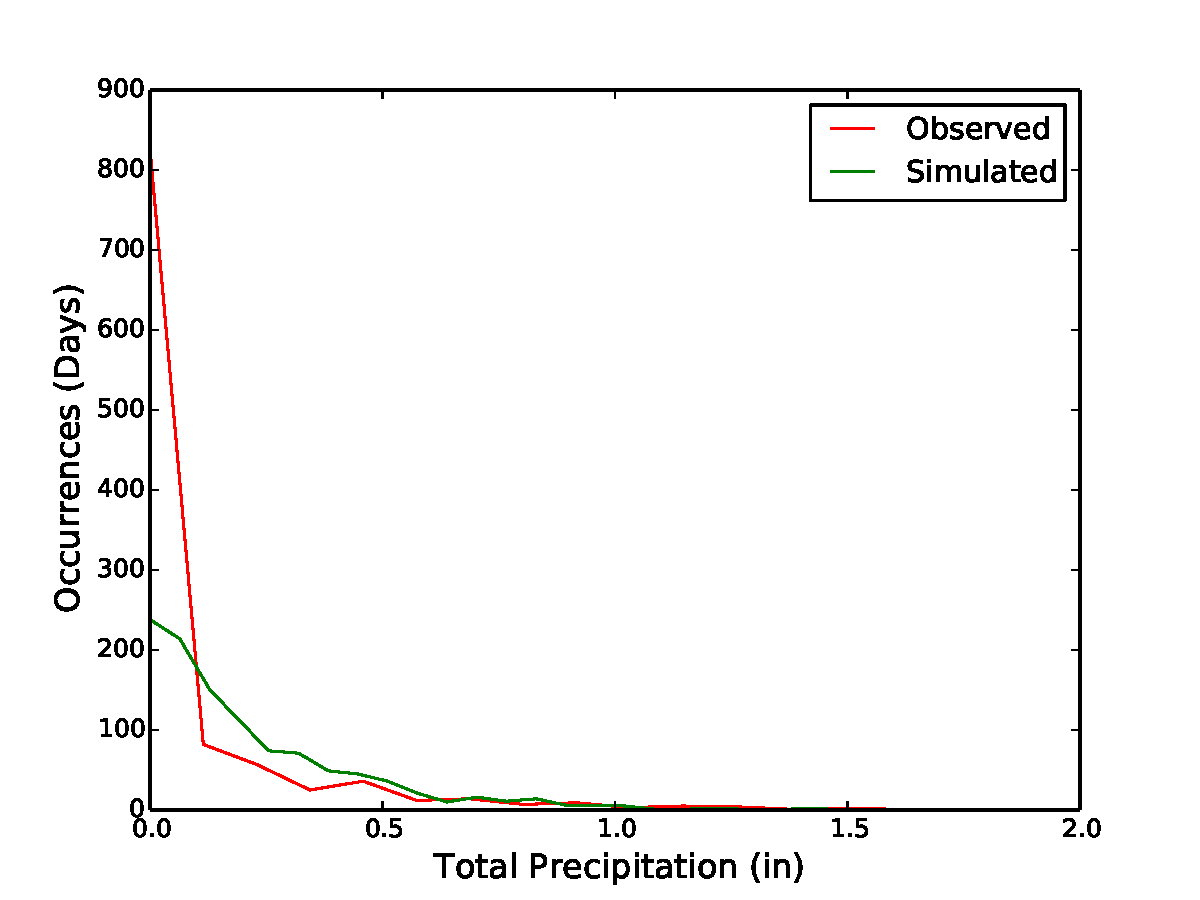
\includegraphics[width=\textwidth]{figures/daily_precip_hist.pdf}
    \caption{Daily Precipitation Histogram}
  \end{subfigure}
  ~
  \begin{subfigure}[b]{0.45\textwidth}
    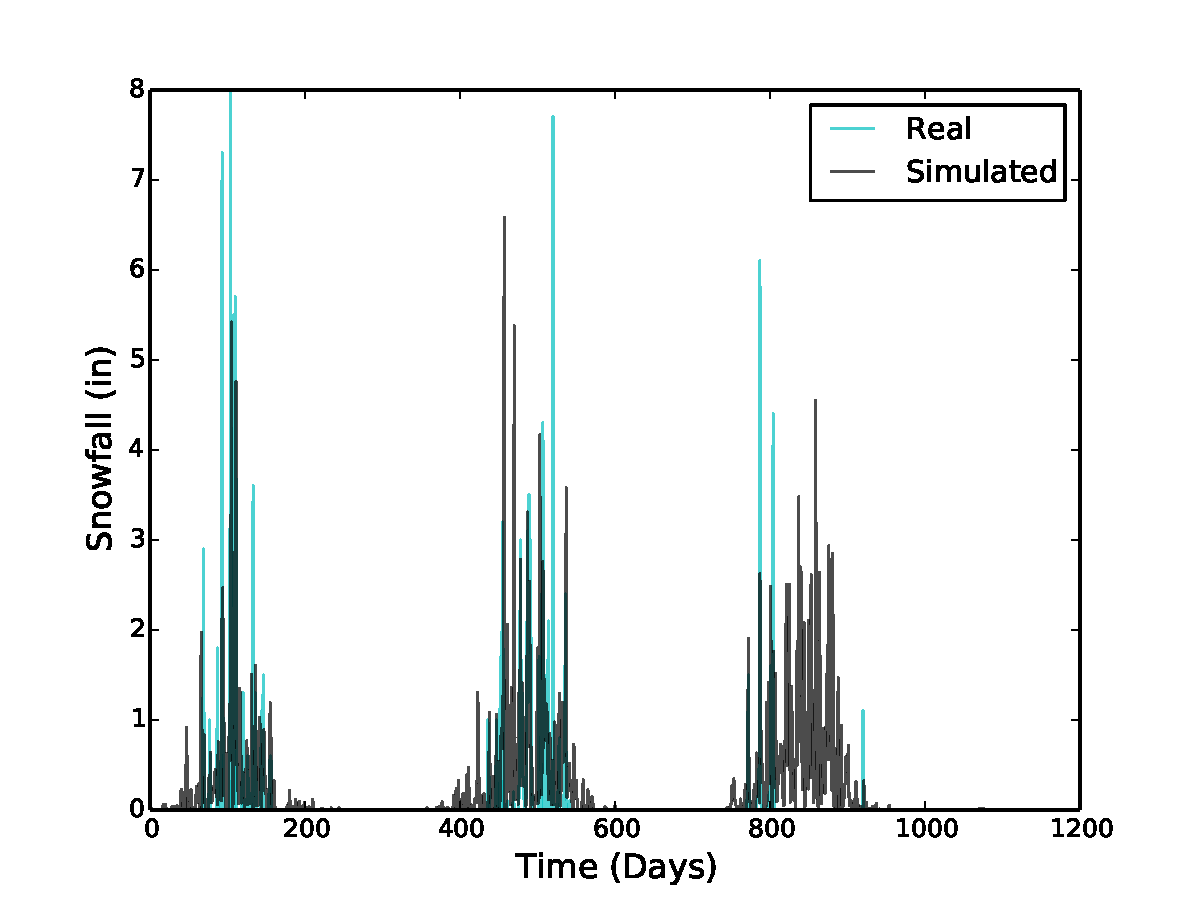
\includegraphics[width=\textwidth]{figures/daily_snowfall.pdf}
    \label{fig:analysis-raw}
    \caption{Daily Snowfall}
  \end{subfigure}
  ~
  \begin{subfigure}[b]{0.45\textwidth}
    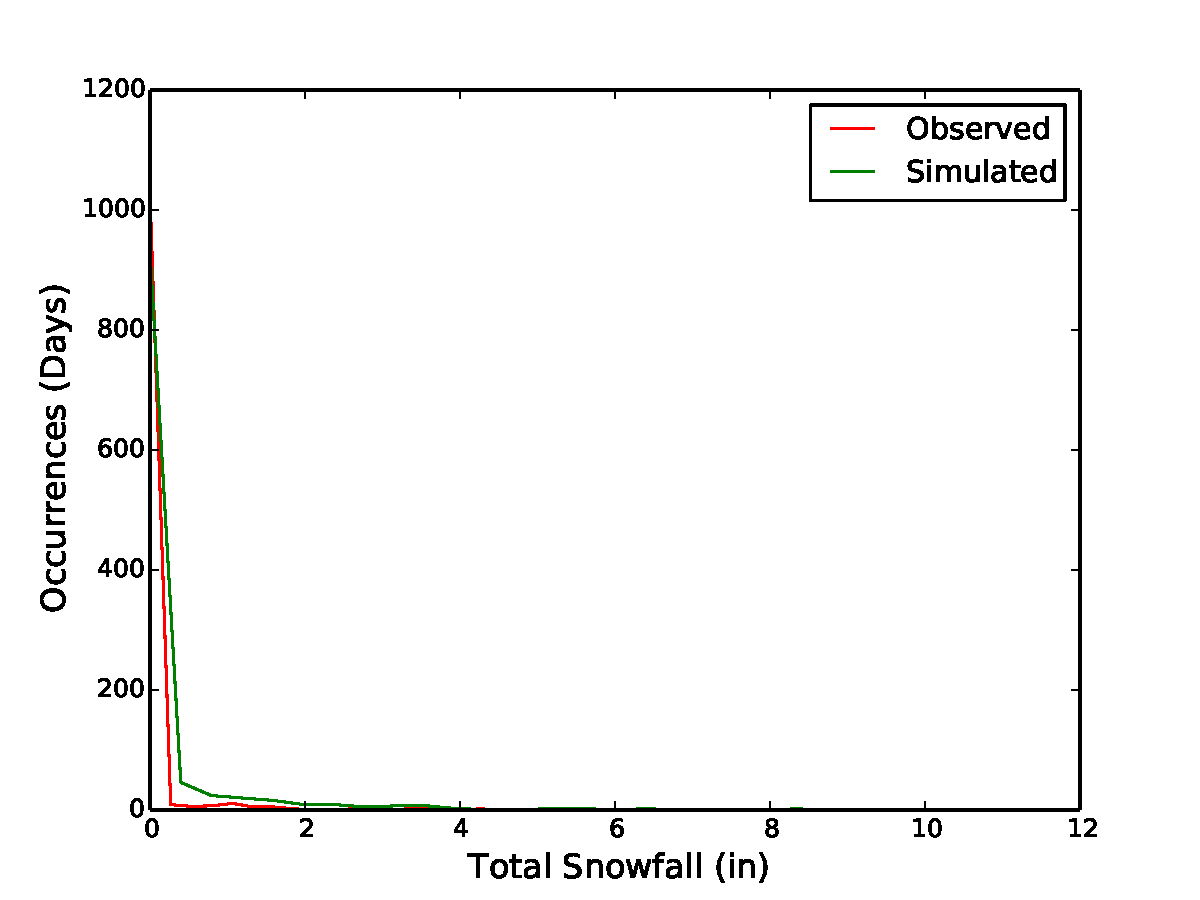
\includegraphics[width=\textwidth]{figures/daily_snowfall_hist}
    \caption{Daily Snowfall Histogram}
  \end{subfigure}
  ~
  \begin{subfigure}[b]{0.45\textwidth}
    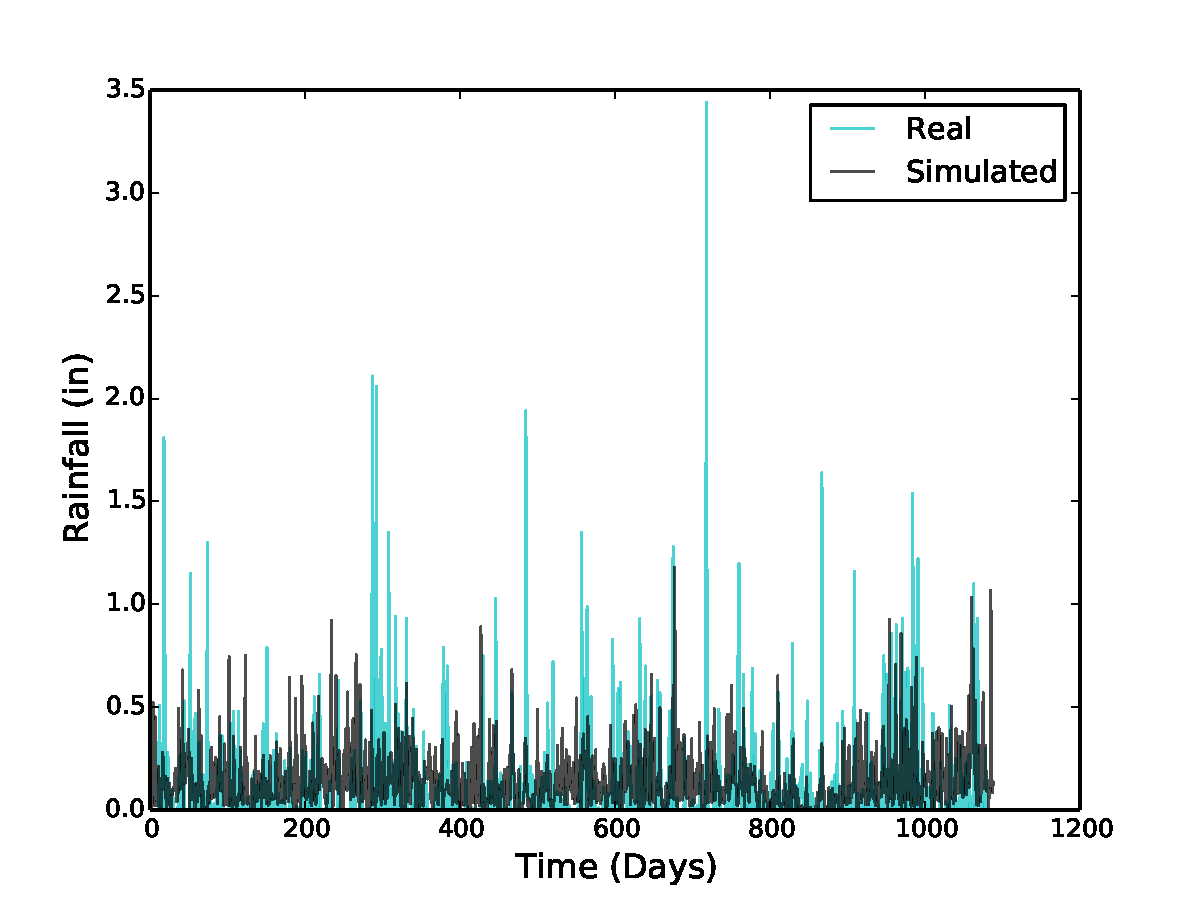
\includegraphics[width=\textwidth]{figures/daily_rainfall.pdf}
    \label{fig:analysis-raw}
    \caption{Daily Rainfall}
  \end{subfigure}
  ~
  \begin{subfigure}[b]{0.45\textwidth}
    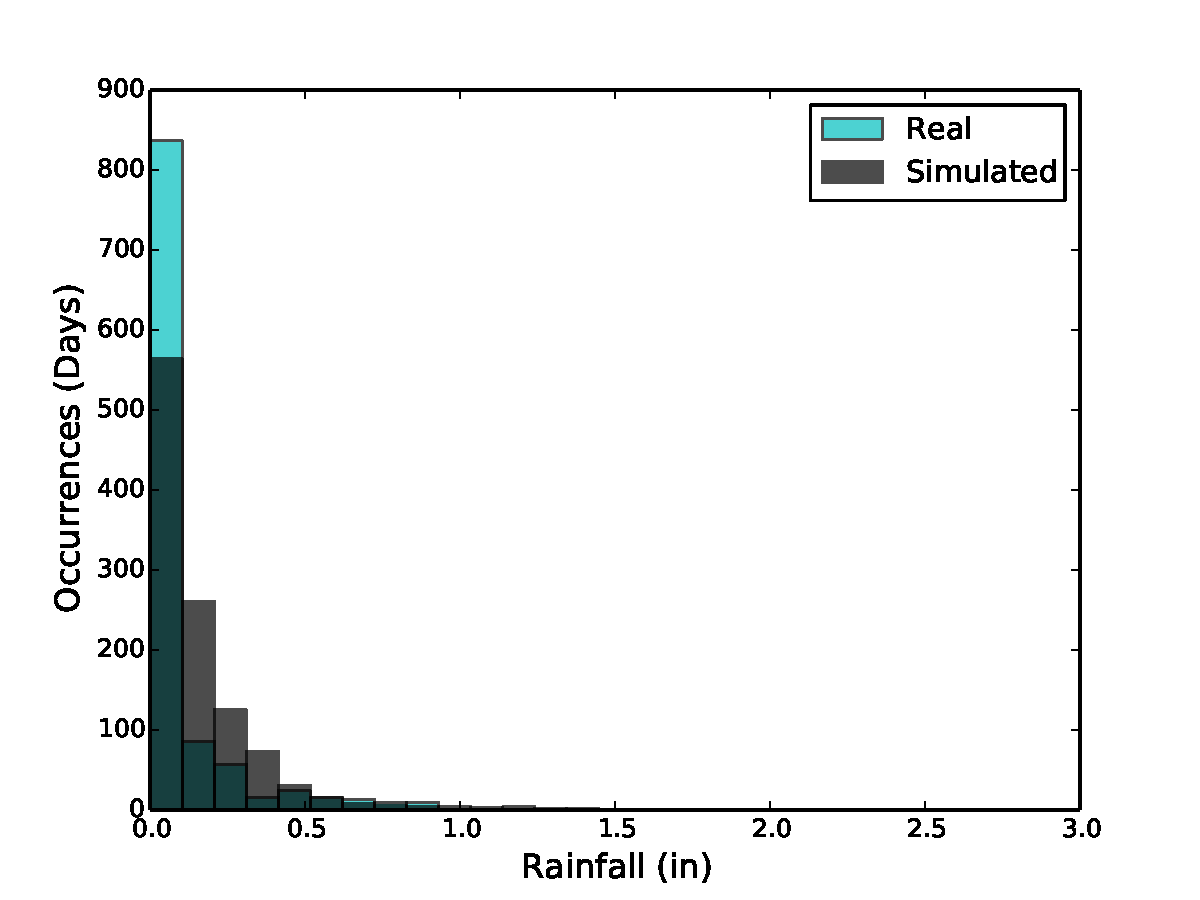
\includegraphics[width=\textwidth]{figures/daily_rainfall_hist}
    \caption{Daily Rainfall Histogram}
  \end{subfigure}
  \label{fig:analysis}
  \caption{}
\end{figure}

\begin{figure}[H]
  \centering
  \begin{subfigure}[b]{0.45\textwidth}
    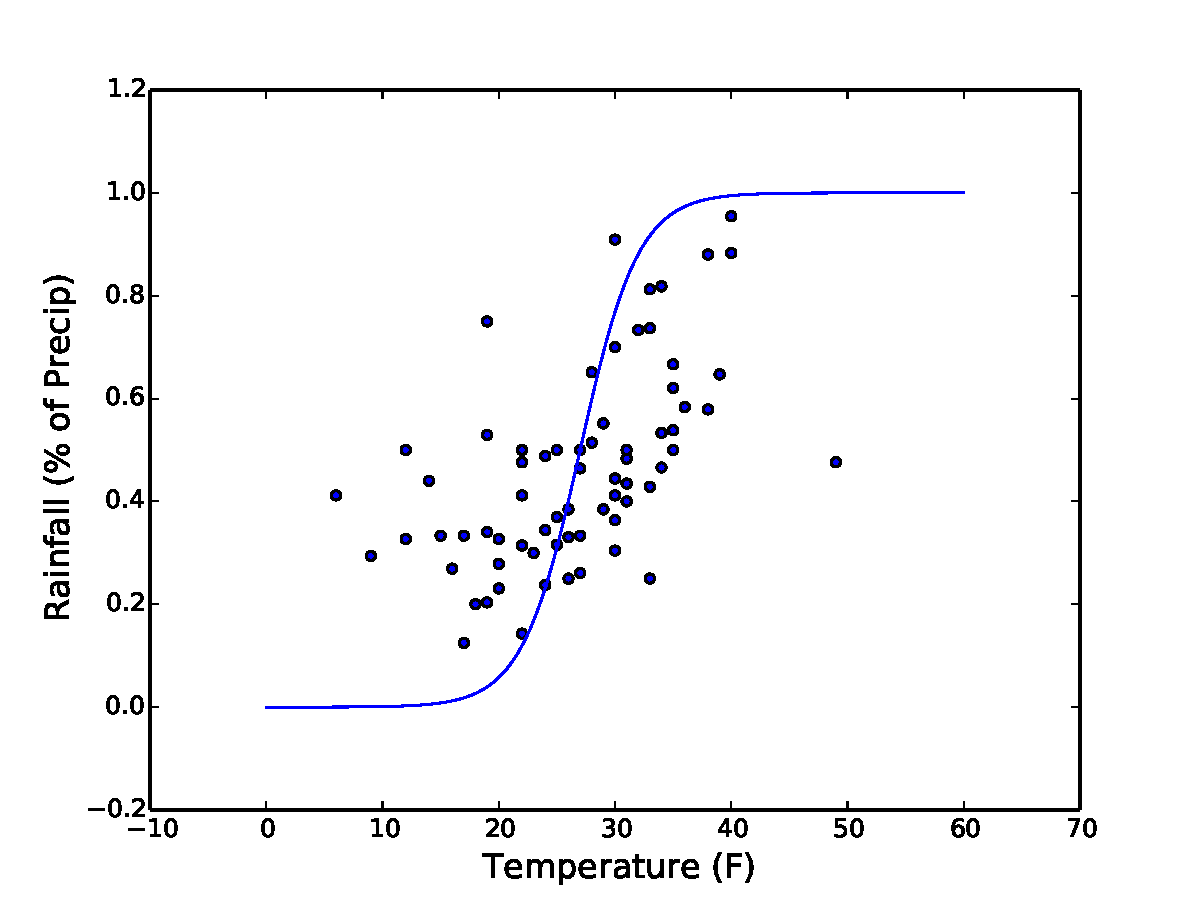
\includegraphics[width=\textwidth]{figures/daily_temp_precip_scatter.pdf}
    \caption{Temperature-Precipitation Scatter}
  \end{subfigure}
  ~
  \begin{subfigure}[b]{0.45\textwidth}
    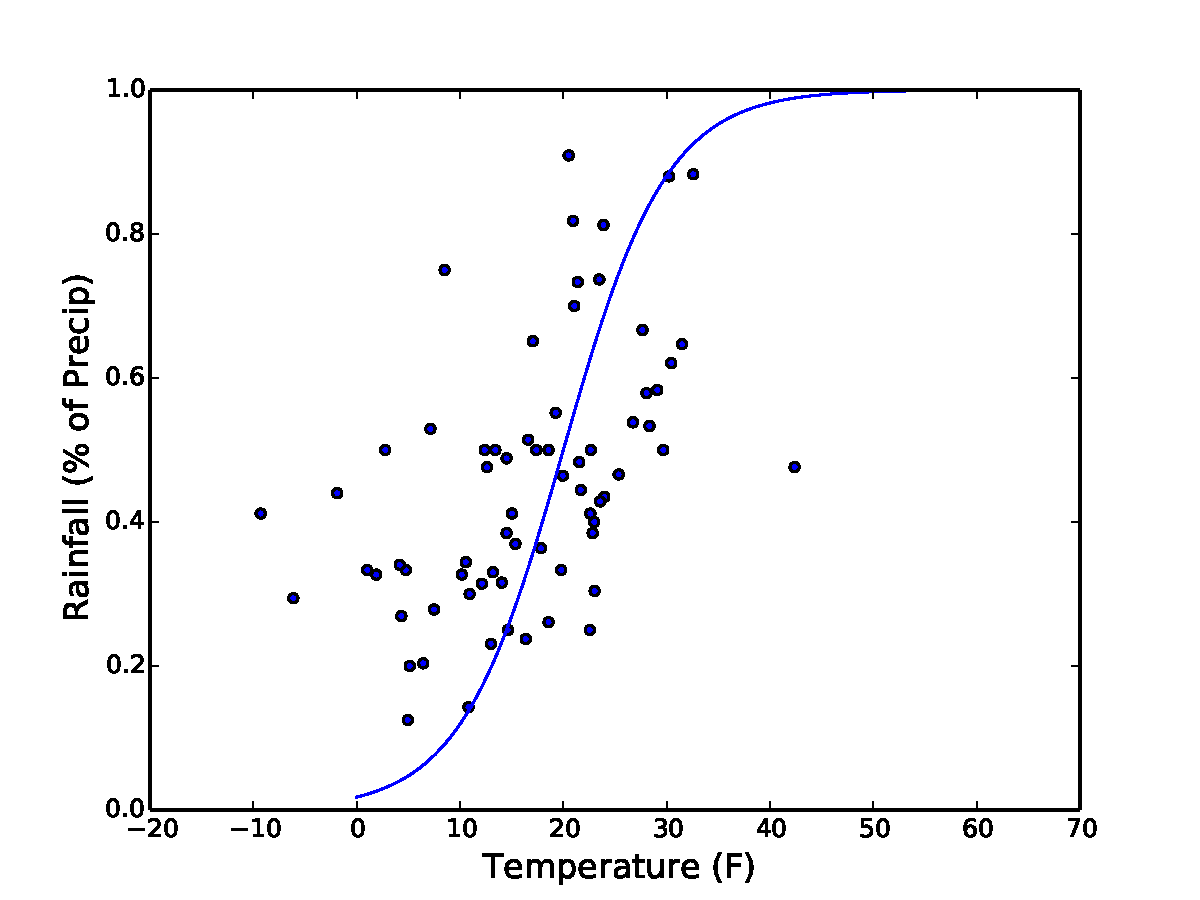
\includegraphics[width=\textwidth]{figures/daily_wind_chill_precip_scatter.pdf}
    \caption{Wind Chill-Precipitation Scatter}
  \end{subfigure}
  \caption{}
\end{figure}

\textcolor{red}{TODO autocorr, FFT, snowfall graph}

\subsection{Wind}

\subsubsection{Analysis of Raw Data}

\begin{enumerate}
\item The wind process is driven by two components: a single signal in the low-frequency regime with an amplitude $>$ the median amplitude while the other frequencies have amplitudes near the median (FFT).
\item The low-frequency signal is deterministic and sinosidal (autcorrelation).
\item The signals for the remaining frequencies are characterized by a stochastic process (autocorrelation).
\item The derivative of the wind, which is dominated by the white noise, is normally (Gaussian) distributed (derivative value histogram).
\end{enumerate}


\subsubsection{Description of Model}
Based on the properties observed in Section~\ref{sec:analysis}, we can derive a model.

\begin{equation}
\tilde{W}(t) = \frac{1}{2}a_0 + a \sin\Big(\frac{-2.0 \pi n}{P}\Big) + b \cos\Big(\frac{-2.0 \pi n}{P}\Big) + X_t
\end{equation}

\begin{table}[H]
  \centering
  \begin{tabular}{c c} \hline
  \emph{Variable} & \emph{Description}\\ \hline
  $\tilde{W}$ & Simulated wind speed \\ \hline
  $t$ & time \\ \hline
  $a_0$ & average wind speed \\ \hline
  $a$ & \\ \hline
  $b$ &  \\ \hline
  $P$ & period  \\ \hline
  $X_t$ & $X_t \sim$ Erlang distribution \\ \hline 
  \end{tabular}
  \caption{Descriptions of variables in the model}
  \label{tab:analysis-ft-values}
\end{table}

\subsubsection{Implementation of the Model}

\subsubsection{Evaluation of the Model}

\begin{figure}[H]
  \centering
  \begin{subfigure}[b]{0.45\textwidth}
    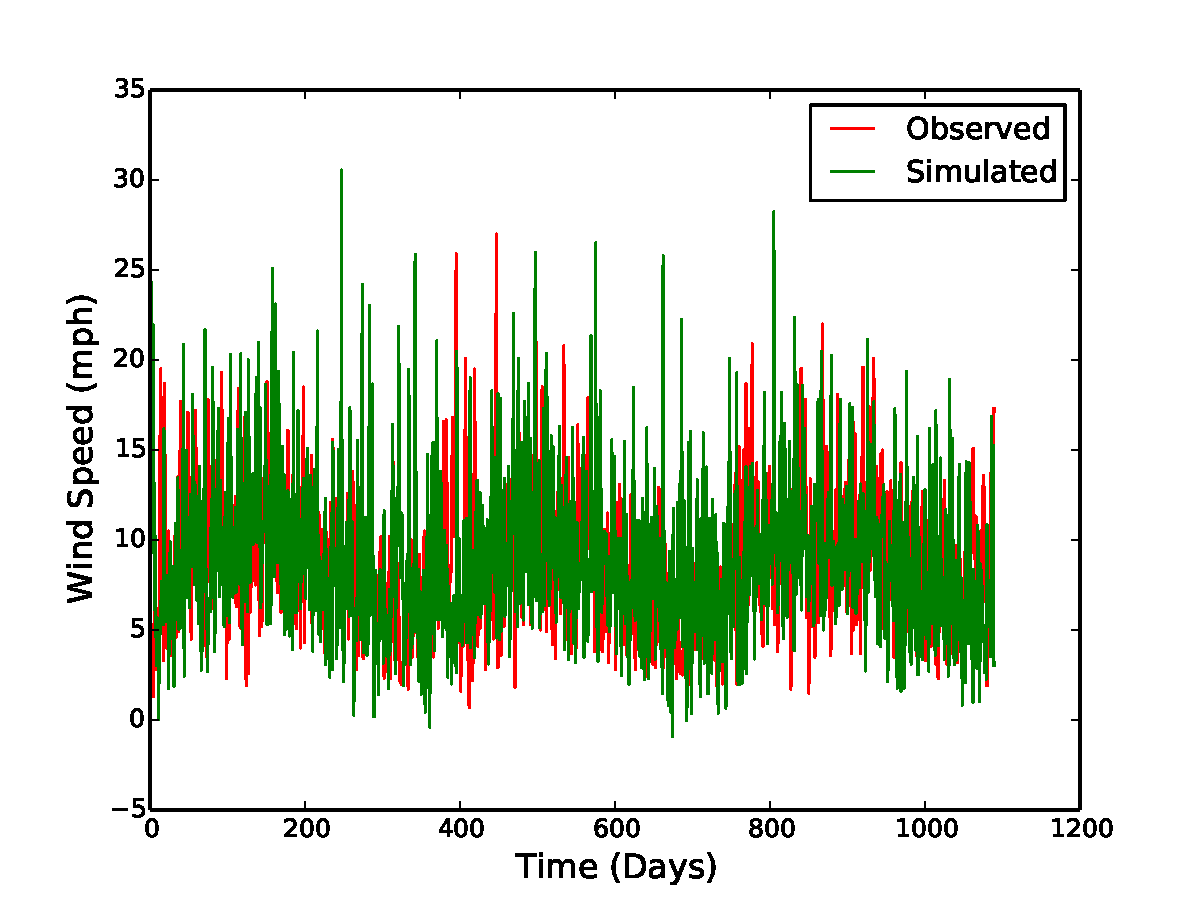
\includegraphics[width=\textwidth]{figures/daily_wind_speeds.pdf}
    \label{fig:analysis-raw}
    \caption{Daily Wind Speed}
  \end{subfigure}
  ~
  \begin{subfigure}[b]{0.45\textwidth}
    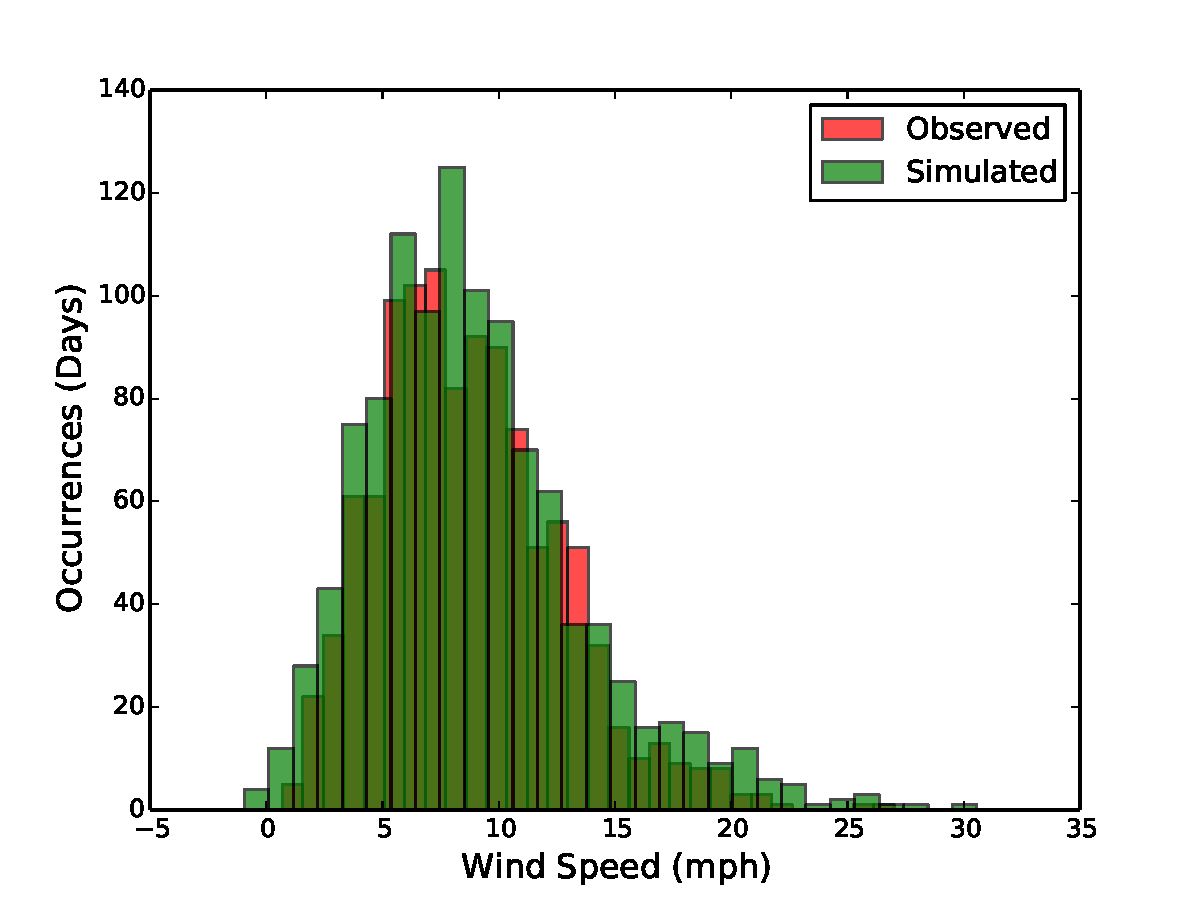
\includegraphics[width=\textwidth]{figures/daily_wind_speed_hist.pdf}
    \caption{Daily Wind Speed Histogram}
  \end{subfigure}
  ~
  \begin{subfigure}[b]{0.45\textwidth}
    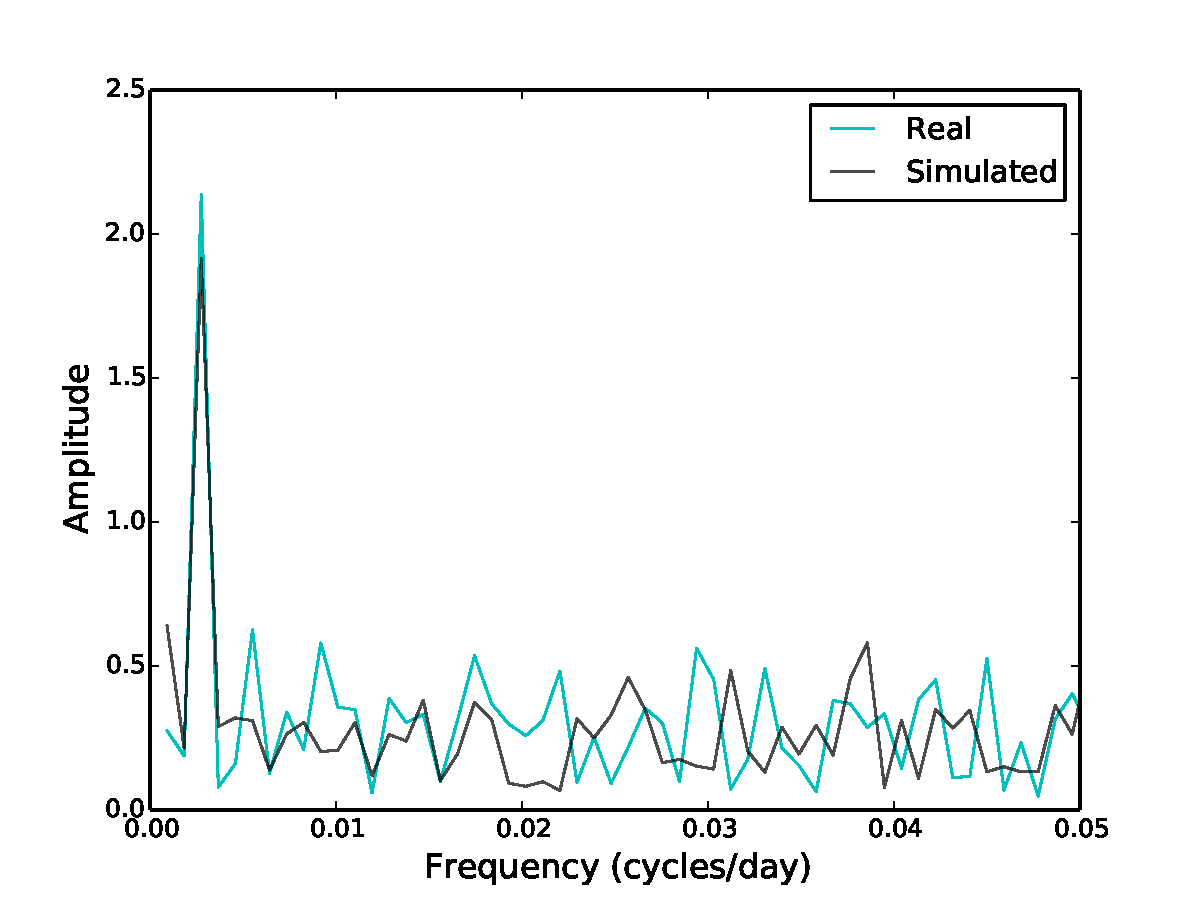
\includegraphics[width=\textwidth]{figures/daily_wind_speed_fft.pdf}
    \caption{Wind Speed FT}
  \end{subfigure}
  
  \label{fig:analysis}
  \caption{}
\end{figure}


\subsection{Review of Other Weather Models}

\newpage
\section{Proposed Modifications to Transaction and Purchasing Models}

\subsection{Determination of Weather Quality}

Need models to quantify ``quality'' of weather as a value in $[0, 1]$ where 1 indicates the best possible weather and 0 indicates the worst possible weather.  Weather quality could be modeled separately for temperature, snow fall, rain fall, and wind and combined using a ``min'' operator.   

Based on the weather quality for each day, we would need to model the probability of a customer going shopping given the weather conditions.

\begin{equation}
q_T(T) = \frac{1 - c}{1 + \exp(-a (T - b))} + c
\end{equation}

\begin{equation}
q_s(s) = 1 - \frac{1 - c}{1 + \exp(-a (s - b))}
\end{equation}



\begin{figure}[H]
  \centering
  \begin{subfigure}[b]{0.45\textwidth}
    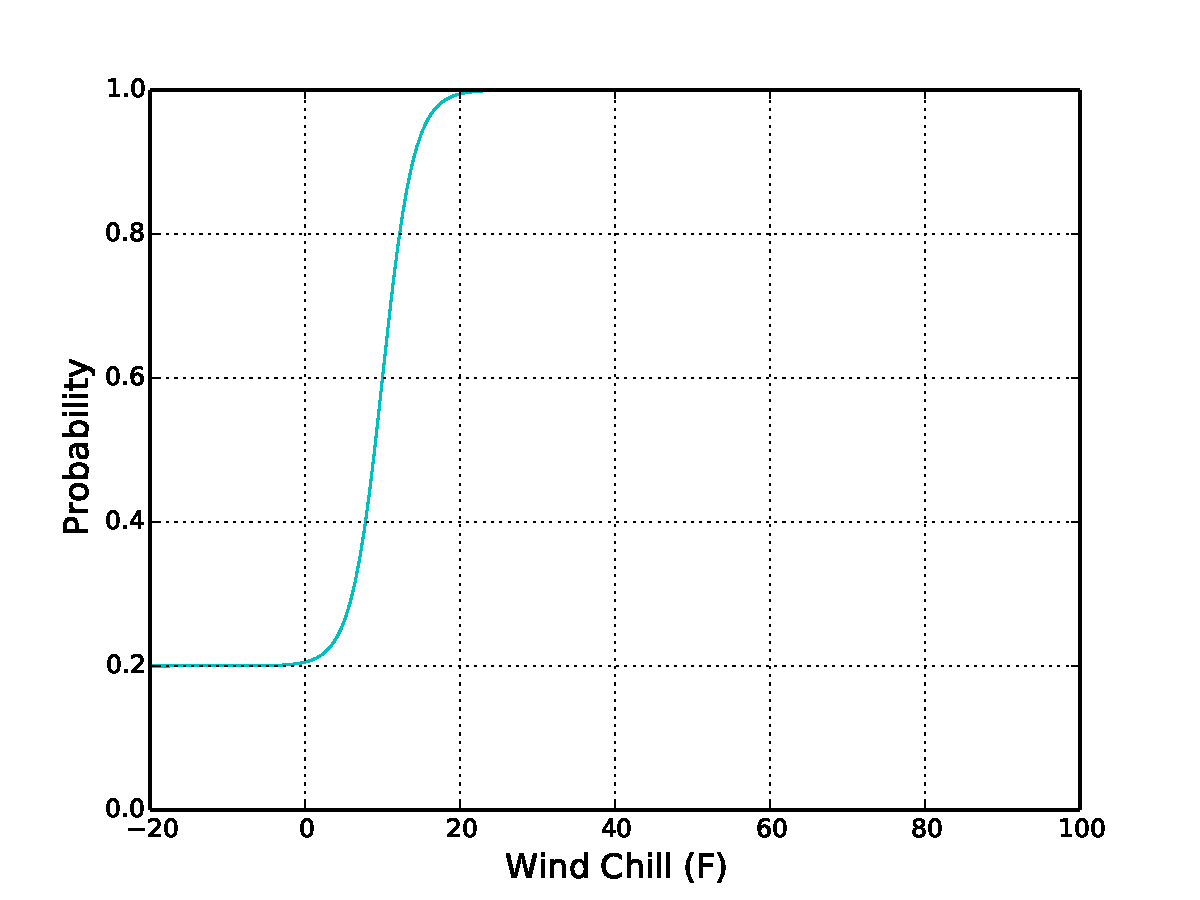
\includegraphics[width=\textwidth]{figures/wind_chill_trans_prob.pdf}
    \label{fig:analysis-raw}
    \caption{Wind Chill Transaction Probabilities}
  \end{subfigure}
  ~
  \begin{subfigure}[b]{0.45\textwidth}
    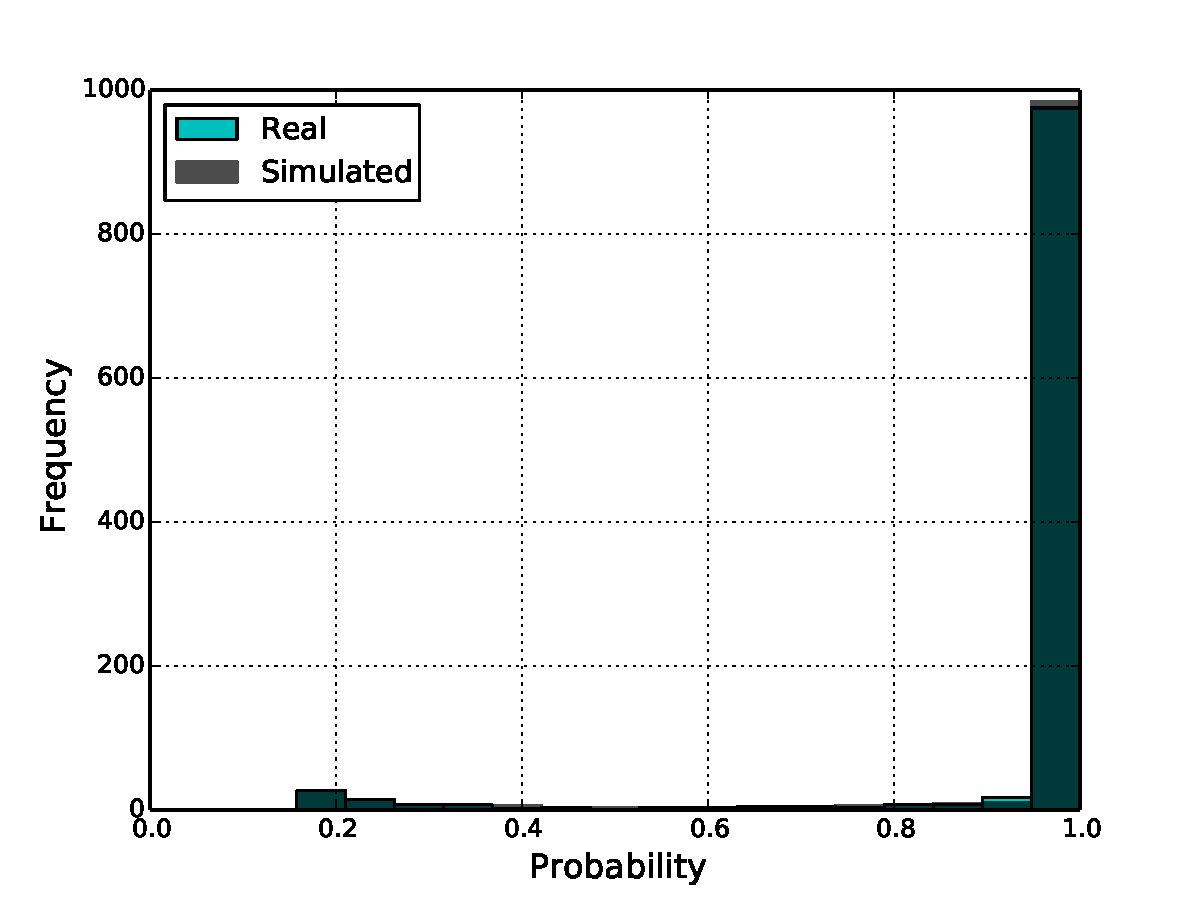
\includegraphics[width=\textwidth]{figures/wind_chill_trans_prob_hist.pdf}
    \caption{Wind Chill Trans. Prob. Histogram}
  \end{subfigure}
  ~
  \begin{subfigure}[b]{0.45\textwidth}
    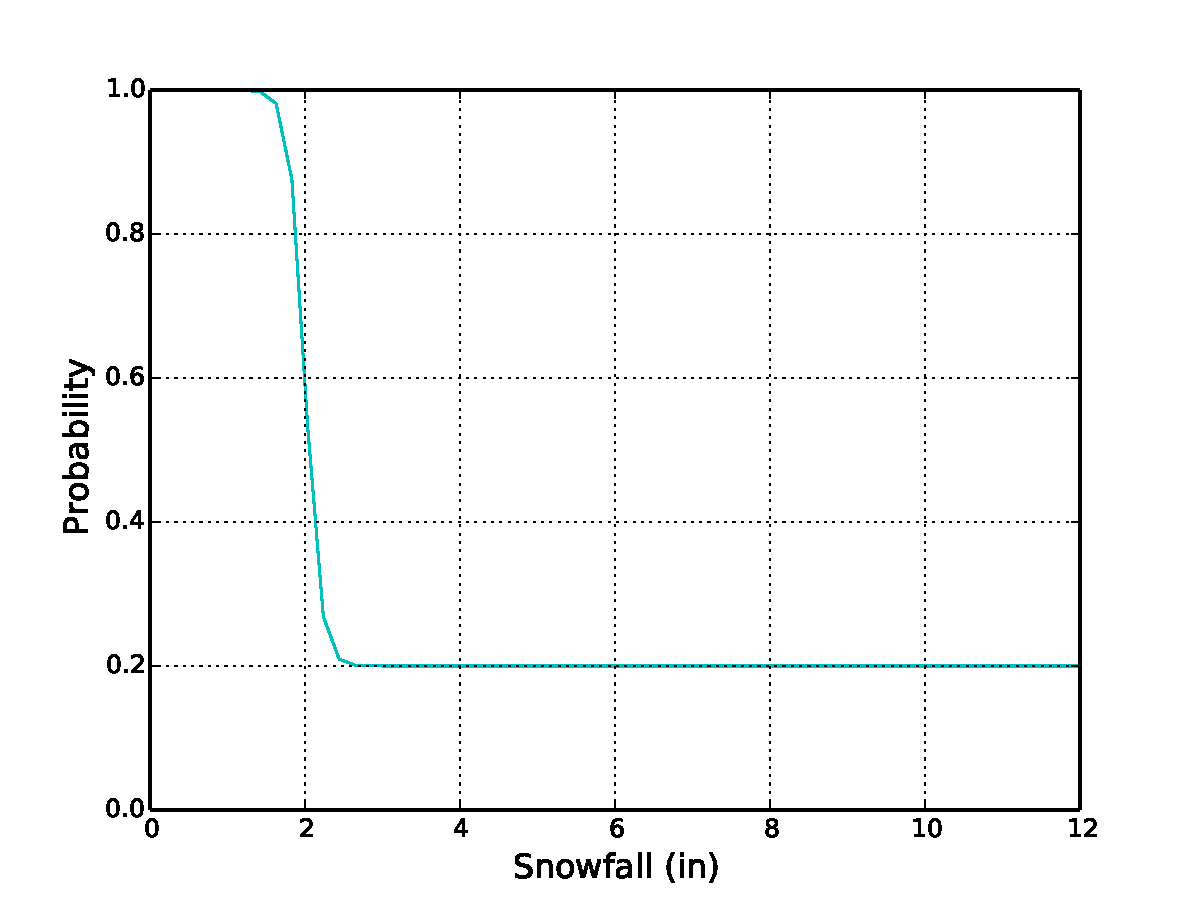
\includegraphics[width=\textwidth]{figures/snowfall_trans_prob.pdf}
    \label{fig:analysis-raw}
    \caption{Snowfall Transaction Probability}
  \end{subfigure}
  ~
  \begin{subfigure}[b]{0.45\textwidth}
    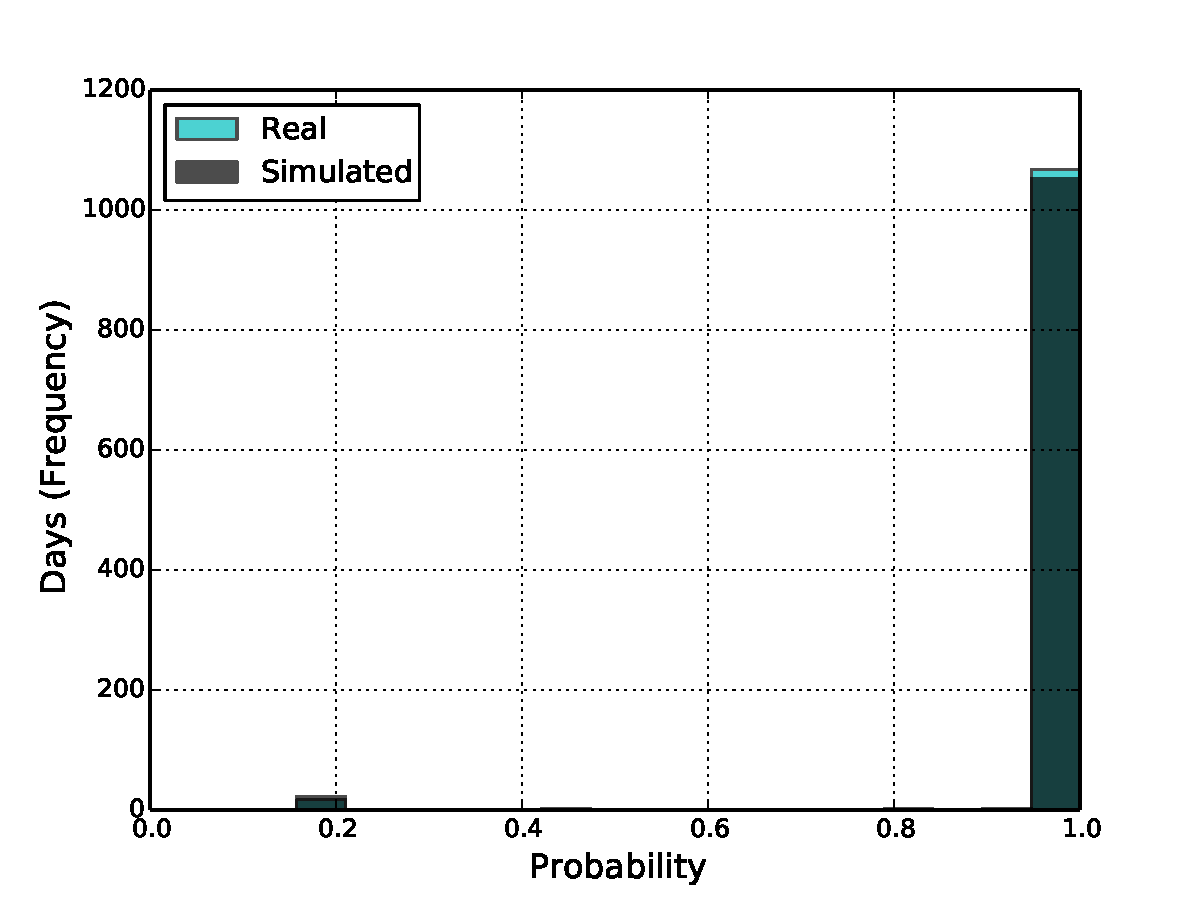
\includegraphics[width=\textwidth]{figures/snowfall_trans_prob_hist.pdf}
    \caption{Snowfall Trans. Prob. Histogram}
  \end{subfigure}
  ~
  \begin{subfigure}[b]{0.45\textwidth}
    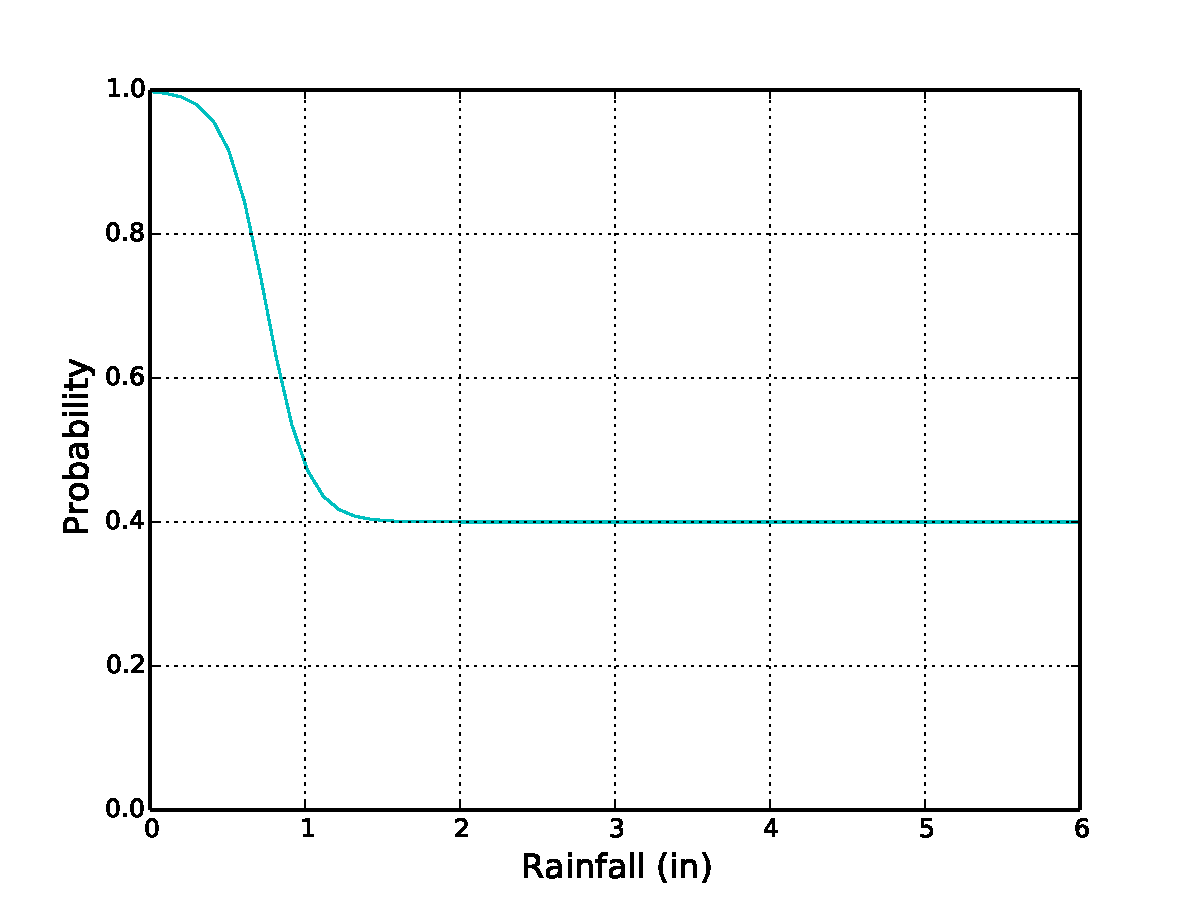
\includegraphics[width=\textwidth]{figures/rainfall_trans_prob.pdf}
    \label{fig:analysis-raw}
    \caption{Rainfall Transaction Probability}
  \end{subfigure}
  ~
  \begin{subfigure}[b]{0.45\textwidth}
    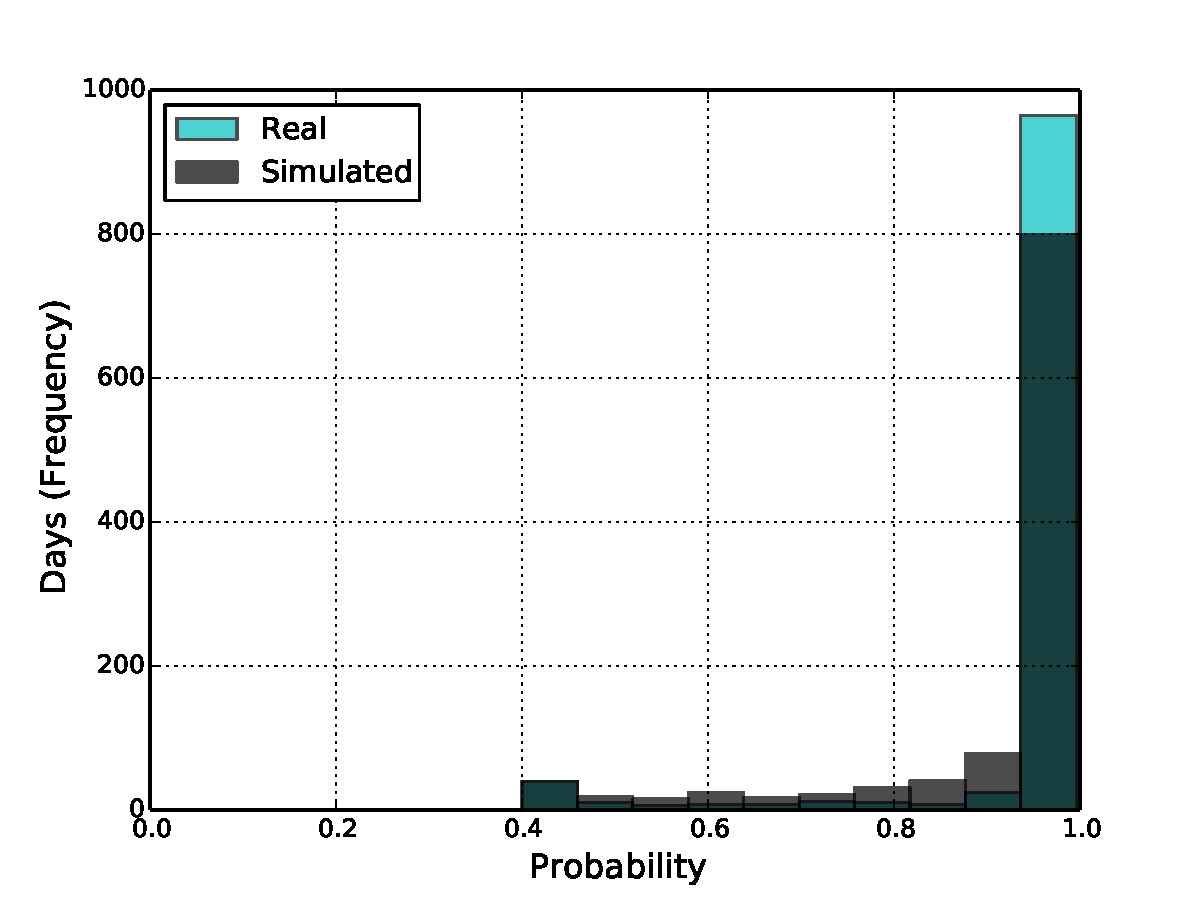
\includegraphics[width=\textwidth]{figures/rainfall_trans_prob_hist.pdf}
    \caption{Rainfall Trans. Prob. Histogram}
  \end{subfigure}
  \label{fig:analysis}
  \caption{}
\end{figure}

\begin{figure}[H]
  \centering
  \begin{subfigure}[b]{0.45\textwidth}
    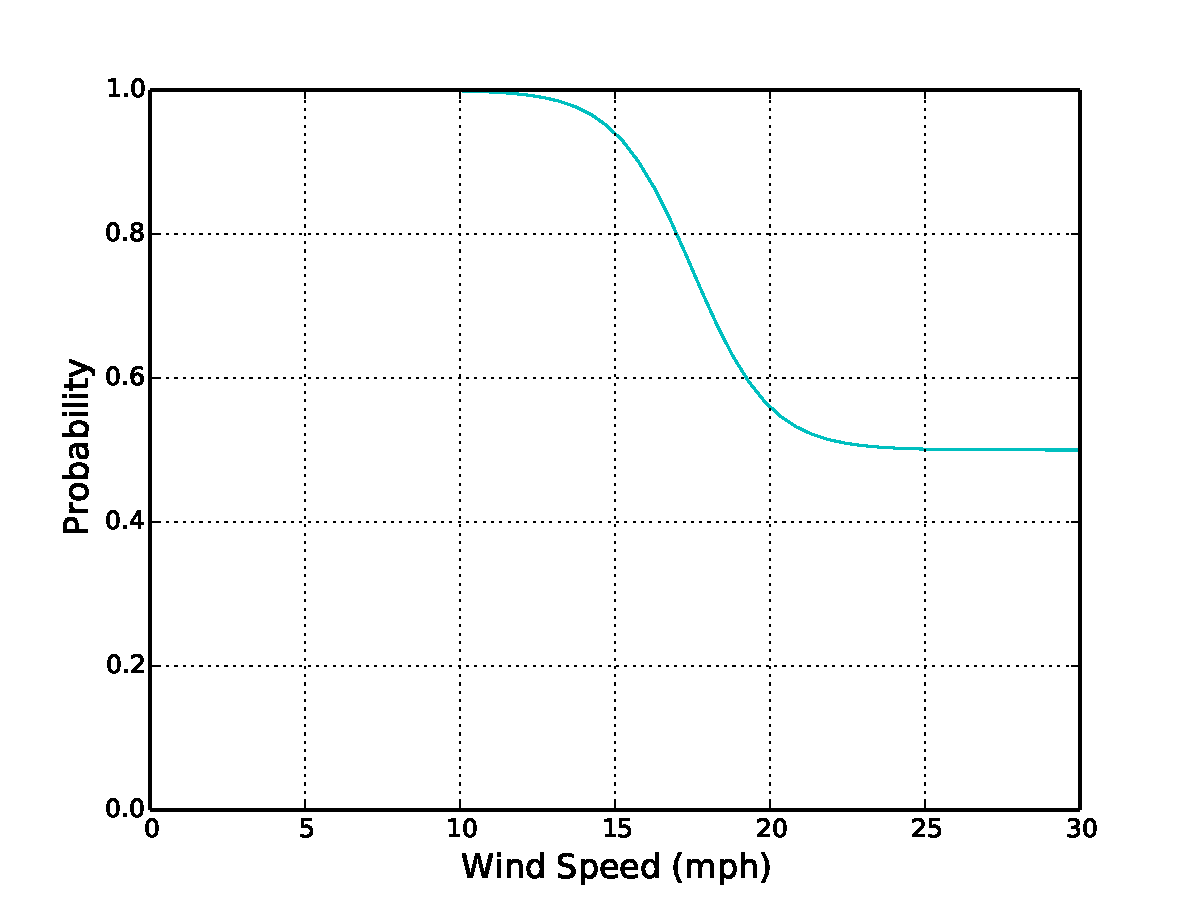
\includegraphics[width=\textwidth]{figures/wind_speed_trans_prob.pdf}
    \label{fig:analysis-raw}
    \caption{Wind Speed Transaction Probability}
  \end{subfigure}
  ~
  \begin{subfigure}[b]{0.45\textwidth}
    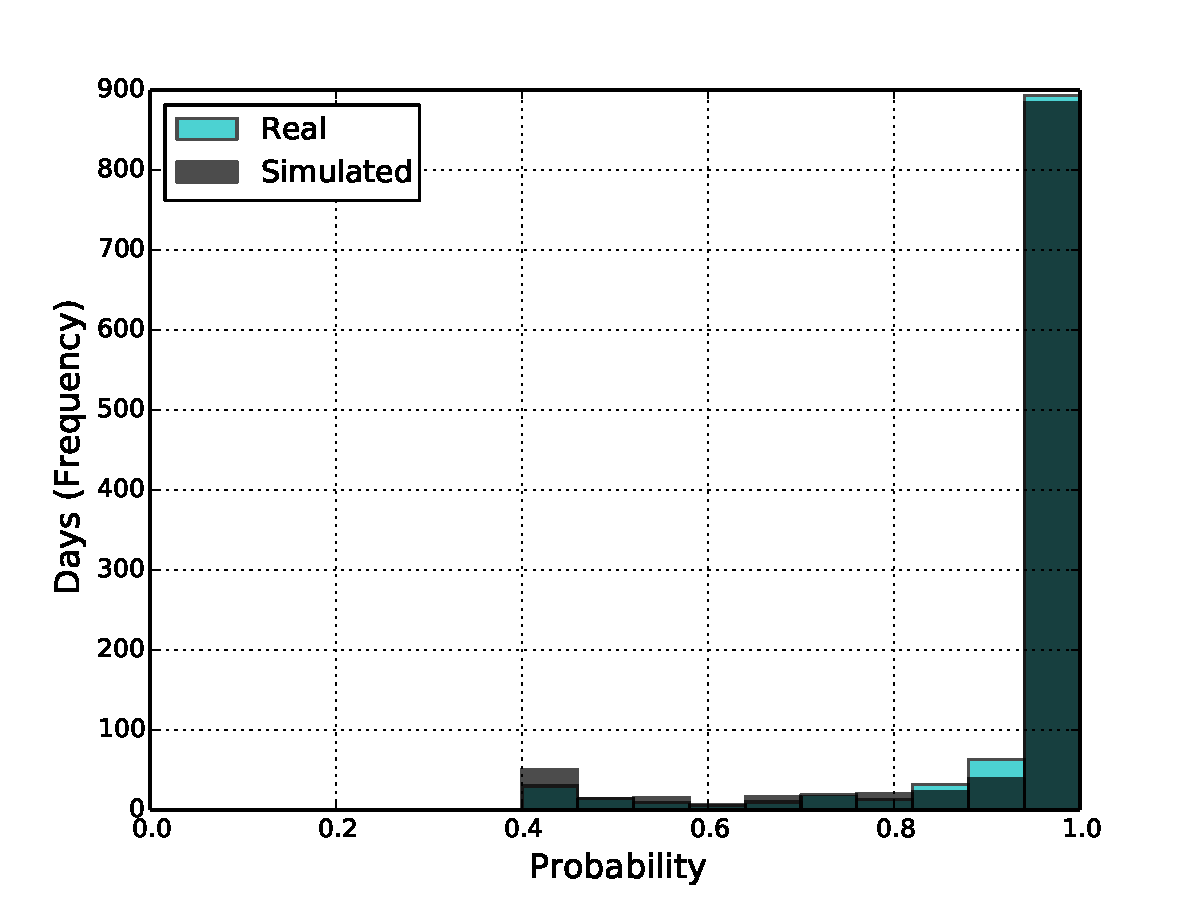
\includegraphics[width=\textwidth]{figures/wind_speed_trans_prob_hist.pdf}
    \caption{Wind Speed Trans. Prob. Histogram}
  \end{subfigure}
  ~
  \begin{subfigure}[b]{0.45\textwidth}
    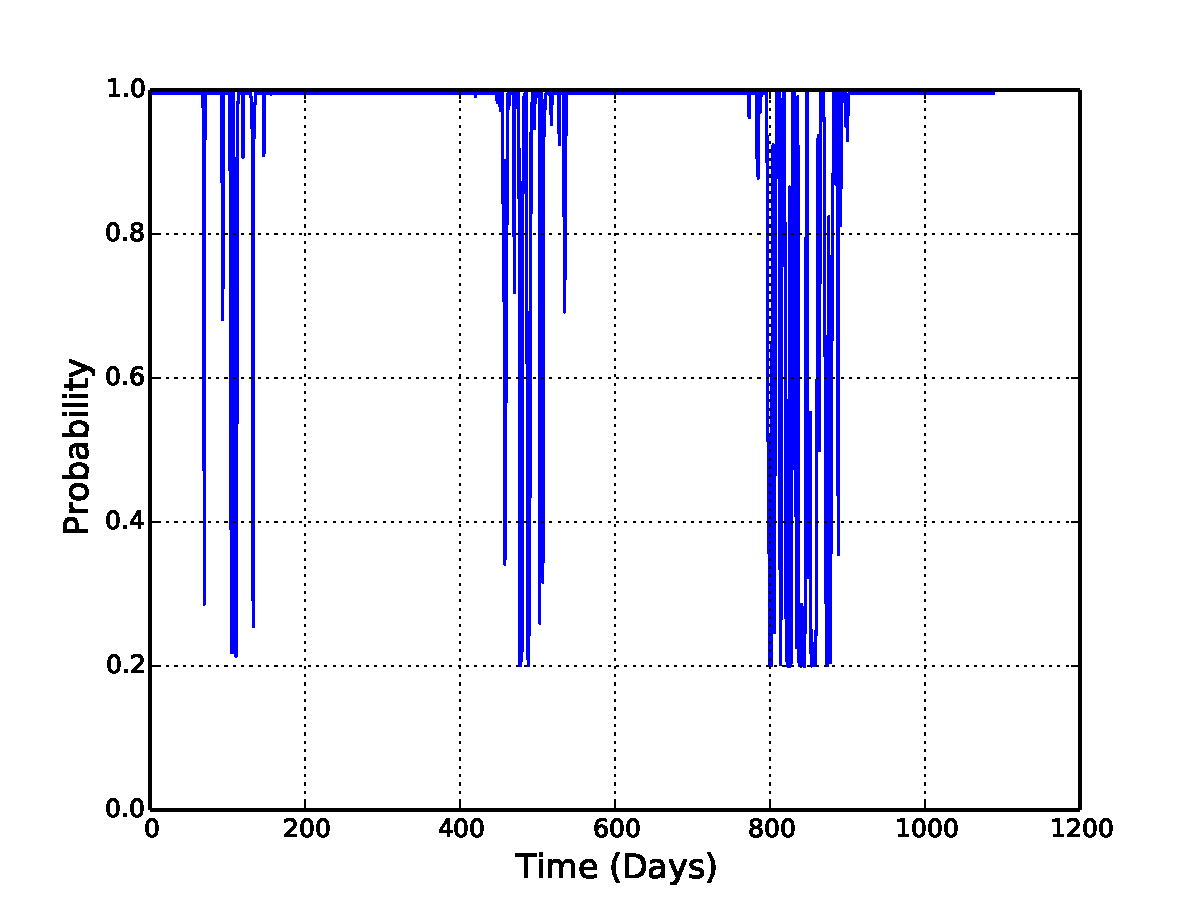
\includegraphics[width=\textwidth]{figures/weather_trans_prob.pdf}
    \caption{Weather Trans. Prob.}
  \end{subfigure}
  \label{fig:analysis}
  \caption{}
\end{figure}



\textcolor{red}{TODO quality vs day, total precipitation, windchill}

\subsection{Transaction Model}

\subsubsection{Review of Existing Model}

\subsubsection{Proposed Changes to Model}

Assumptions:
\begin{enumerate}
\item The probability of customers going to the store on a particular day is decreased under bad weather conditions.
\end{enumerate}

\begin{equation}
p(\text{trans} | t_i) = \frac{p_(\text{trans} | t_i, \text{weather}) \, p_{\text{exhaustion offset}}(\text{trans} | t_i) \, p_{\text{arrow of time}}(\text{trans} | t_i \geq t_{i-1})}{Z}
\end{equation}

\subsubsection{Evaluation of Changes}

\subsection{Purchasing Model}

\subsubsection{Review of Existing Model}

\subsubsection{Proposed Changes to Model}

Assumptions:
\begin{enumerate}
\item Customers will buy larger quantities if they anticipate bad weather coming
\end{enumerate}

Ideas:
\begin{enumerate}
\item Add additional term to category weight functions based on amount of bad weather in the next $N$ days.
\item Increase preferences for larger sizes
\end{enumerate}

\subsubsection{Evaluation of Changes}

\section{Conclusion}


%\bibliography{thesis}
%\bibliographystyle{abbrv}

\end{document}
